\documentclass[pdflatex,sn-nature]{sn-jnl}% Style for submissions to Nature Portfolio journals

\usepackage{graphicx}%
\usepackage{multirow}%
\usepackage{amsmath,amssymb,amsfonts}%
\usepackage{amsthm}%
\usepackage{mathrsfs}%
\usepackage[title]{appendix}%
\usepackage{xcolor}%
\usepackage{textcomp}%
\usepackage{manyfoot}%
\usepackage{booktabs}%
\usepackage{threeparttable}
\usepackage{siunitx}
\usepackage{caption}
\usepackage{algorithm}%
\usepackage{algorithmicx}%
\usepackage{algpseudocode}%
\usepackage{listings}%
\usepackage{hyperref}%
\usepackage{placeins}%

%%%%
\theoremstyle{thmstyleone}%
\newtheorem{theorem}{Theorem}%  meant for continuous numbers
%%\newtheorem{theorem}{Theorem}[section]% meant for sectionwise numbers
%% optional argument [theorem] produces theorem numbering sequence instead of independent numbers for Proposition
\newtheorem{proposition}[theorem]{Proposition}% 
%%\newtheorem{proposition}{Proposition}% to get separate numbers for theorem and proposition etc.
\newcommand{\norm}[1]{\left\|#1\right\|}
\theoremstyle{thmstyletwo}%
\newtheorem{example}{Example}%
\newtheorem{remark}{Remark}%

\theoremstyle{thmstylethree}%
\newtheorem{definition}{Definition}%

\raggedbottom
%%\unnumbered% uncomment this for unnumbered level heads

\begin{document}

\title[Integrating Fundamental Knowledge and Sensor Data: Physics-Informed Neural Networks for Smart Agricultural Water Management]{Integrating Fundamental Knowledge and Sensor Data: Physics-Informed Neural Networks for Smart Agricultural Water Management}






\author*[1]{\fnm{Gregory} \sur{Conde}}\email{gregory.condemen@ufl.edu}

\author[1]{\fnm{Sandra M.} \sur{Guzmán}}\email{sandra.guzmangut@ufl.edu}

\author[2]{\fnm{Jorge I.} \sur{Poveda}}\email{jipoveda@ucsd.edu}

\author[3]{\fnm{Flavia T.} \sur{Zambon}}\email{f.zambon@ufl.edu}


\affil*[1]{\orgdiv{Agricultural and Biological Engineering, Indian River Research and Education Center}, \orgname{University of Florida}, \orgaddress{\city{Fort Pierce}, \postcode{34945}, \state{Florida}, \country{USA}}}

\affil[2]{\orgdiv{Department of Electrical and Computer Engineering}, \orgname{University of California}, \orgaddress{\city{San Diego}, \postcode{92093}, \state{California}, \country{USA}}}

\affil[3]{\orgdiv{Institute of Food and Agricultural Sciences, Indian River Research and Education Center}, \orgname{University of Florida}, \orgaddress{\city{Fort Pierce}, \postcode{34945}, \state{Florida}, \country{USA}}}



%%==================================%%
%% Sample for unstructured abstract %%
%%==================================%%
\abstract{Agriculture accounts for 70\% of global freshwater use, yet irrigation inefficiency threatens food security as water scarcity intensifies. Accurate soil moisture prediction for decision-making is crucial for sustainable water management in horticultural systems; however, traditional approaches face an unresolved challenge: analytical models require site-specific constitutive calibration, while unconstrained data-driven methods can violate physical sign and monotonicity laws needed for reliable predictive control decisions. Here, we present a physics-informed neural network (PINN) that addresses this by embedding the principles of Richards' equation into a deep learning architecture, enabling control-oriented modeling and decision-making in irrigation systems. The PINN discretizes Richards' equation spatially, modeling flow through physically regularized neural branches that yield ordinary differential equations at sensor depths. Trained in two stages—derivative-matching initialization followed by closed-loop fourth-order Runge--Kutta (RK4) trajectory refinement—the model predicts soil moisture across six depths (5--55~\si{cm}) in a commercial Florida citrus block with an overall 3-day held-out forecast RMSE of \SI{1.23}{\%VWC} ($R^2 = 0.807$, Pearson $r = 0.921$, $p = \num{7.94e-178}$; \SI{3.22}{mm} integrated over the 60-\si{cm} profile) while simultaneously inferring depth-resolved evapotranspirative depletion. Across 30 rolling 3-day unseen windows, a 7-day horizon sensitivity check, and physical Jacobian admissibility audits, the proposed PINN reduces 3-day forecast error by 35.6\% over persistence, outperforms single-stage and unregularized ablations, and eliminates the unphysical control-sign inversions (33\%--97\%) exhibited by unconstrained linear and black-box Neural ODE baselines, providing an interpretable model suitable for future model-predictive irrigation control.}

%\keywords{Water, Smart Irrigation, Physics Informed Neural Networks, PINN, Modeling, Soil Moisture, Richards' equation}





\maketitle

Agriculture consumes 70\% of global freshwater\cite{scanlon2023}, yet irrigation efficiency remains below 50\% in many regions\cite{Mehta2024}, resulting in the wasteful use of a resource essential for food security. Throughout this work, soil moisture (SM) and soil water content (SWC) are quantified on a volumetric basis as volumetric water content (\si{\%VWC}), defined as the volume of liquid water per bulk volume of soil ($\mathrm{cm^3\,cm^{-3}} \times 100$); for a \SI{10}{cm} vertical soil compartment, \SI{1}{\%VWC} corresponds directly to \SI{1}{mm} of equivalent water depth. Potential atmospheric evaporative demand is quantified by the reference evapotranspiration $ET_0$ (\si{mm/h}), computed from meteorological measurements via the FAO-56 Penman--Monteith equation~\cite{allen1998crop}. Smart irrigation systems, which utilize sensors and algorithms to optimize water delivery, offer a solution; however, while recent machine-learning, time-series, and water-balance frameworks have begun integrating historical SWC, weather variables, and uncertainty estimates for multi-depth forecasting and irrigation scheduling~\cite{Zou2010, Bagheri2025, condeforecast2024}, developing multi-depth models that simultaneously preserve physical consistency (e.g., non-negative drainage and monotonic forcing response) and retain direct structural suitability for model predictive control (MPC) remains challenging. The result is irrigation management that remains largely reactive rather than anticipatory, missing opportunities to reduce water use while maintaining crop productivity.

%--- Move 2: Practical & Scientific Gaps --------------------------------------

The technical gap is well-defined. Smart irrigation algorithms are necessary to pinpoint the precise locations where water should be supplied as plant root systems develop. During germination, water must reach the topsoil layers where seeds are planted; as crops develop, deeper soil layers become critical. Although studies provide general depth guidelines for certain crop types \cite{ASABE2021}, the ability to precisely locate where plants require water based on real-time crop data remains elusive. Algorithms must account for how irrigation, rainfall, plant water uptake, and environmental conditions collectively influence soil water content (SWC) across depths, ideally integrating weather forecasts to predict soil moisture response to upcoming irrigation events. Current approaches fall short: one method uses potential evapotranspiration and crop coefficients to calculate water requirements \cite{Volk2024}; another irrigates based on sensor thresholds between field capacity and maximum allowable depletion \cite{zhang2021}, whereas control-oriented MHE/MPC formulations~\cite{condeforecast2024} typically aggregate the root zone into a lumped single-zone water-balance compartment, and existing multi-depth data-assimilation or sequence-learning hybrids~\cite{Zou2010, Jiang2025, Jiang2026} omit explicit irrigation actuation ODE branches.
The modeling challenge is formidable. Capturing plant-soil-water interactions at multiple depths requires confronting: (i) the dynamic nature of plant growth and water uptake, which varies with crop type, phenology, and environmental conditions; (ii) the nonlinearity of Richards' equation governing vertical water movement in unsaturated soils, which demands complex numerical methods \cite{Celia1990}; (iii) the empirical constitutive models (e.g., Gardner, van Genuchten, Brooks–Corey) that represent gravitational and capillary forces in Richards' equation, requiring labor-intensive parameter calibration and lacking universal applicability across soil types \cite{Pan2019}; and (iv) the coarse spatial and temporal resolution of available data, which forces discretizations that can violate numerical stability criteria \cite{Celia1990,leveque2007}. Traditional analytical models are computationally expensive and require soil hydraulic parameters that vary unpredictably in heterogeneous fields. Purely data-driven machine learning models can predict soil moisture accurately in-distribution, but they produce "black box" outputs that can violate sign and monotonicity conditions with respect to control inputs ($q_{\mathrm{irr}}, ET_0$) and lack the physical consistency and stability guarantees necessary for model predictive control.

%--- Move 3: Opportunity & Approach -------------------------------------------
Here, we address this dichotomy with physics-informed neural networks (PINNs), a technique that combines neural network function approximation, machine learning tools, established soil-water dynamics theory, and plant biophysics into models suitable for smart irrigation management. Originally created to reduce computational costs when solving partial differential equations (PDEs)  \cite{Cuomo2022}, PINNs overcome the limitations of purely data-driven approaches (which require vast data and lack physical consistency) and analytical models (which are computationally expensive and depend on system-specific governing equations).


%--- Move 4: Prior Art & Positioning
Recent applications demonstrate the potential of PINNs for control-oriented modeling in high-uncertainty systems, such as automated vehicles and quantum systems \cite{Li2024, Zhang2025}. In soil sciences, PINNs have been explored as alternatives to numerical solutions of Richards' equation \cite{Bandai2022}, for handling sparse data in unsaturated infiltration modeling \cite{Lan2024}, for estimating hydraulic conductivity functions \cite{Elkha2024}, and for predicting SWC \cite{Bagheri2025}. More recently, constitutive neural networks have been embedded in differentiable finite-volume Backward Euler solvers with Newton root-finding on fine grids ($100$ cells on a \SI{10}{cm} lab column; $150$ cells on a \SI{1.5}{m} synthetic profile) \cite{Bandai2024}, and physics-informed operator networks (PI-DeepONet) have mapped 100-day meteorological series to $(z,t)$ profiles \cite{Ye2025}, alongside multi-depth time-series models \cite{Zou2010}, physics-guided LSTM/CNN-LSTM predictors \cite{WangY2023, ZhangT2025, Jiang2026}, EnKF--\texttt{fsolve} assimilation \cite{Jiang2025}, and lumped water-balance MHE/MPC \cite{condeforecast2024} (Table~\ref{tab:lit_comparison}). However, fine-grid implicit PDE surrogates and operator networks omit crop-sink and irrigation actuation channels, sequence networks retain black-box recurrent states, and lumped MPC models lack vertical root-zone resolution. Addressing this gap, the present study contributes: (1) a \emph{sensor-depth finite-volume discretization} of Richards' equation aligned directly with commercial multi-depth probes (5--55~\si{cm}) without fixed van Genuchten/Brooks--Corey curves; (2) \emph{decomposed, physically regularized neural flux branches} ($c_1$--$c_3$) for vertical drainage, signed inter-layer exchange, lateral ditch outflow, rainfall, irrigation, and evapotranspirative depletion; and (3) \emph{two-stage derivative-to-RK4 identification} verified through multi-window benchmarks, ablations, and Jacobian control-admissibility audits.

\begin{table}[!htbp]
\centering
\caption{Positioning of the proposed sensor-depth PINN relative to representative physics-informed soil hydrology and control-oriented smart irrigation studies.}
\label{tab:lit_comparison}
\scriptsize
\setlength{\tabcolsep}{2.5pt}
\begin{tabular}{@{}>{\raggedright\arraybackslash}p{0.165\textwidth}>{\raggedright\arraybackslash}p{0.16\textwidth}>{\raggedright\arraybackslash}p{0.18\textwidth}>{\raggedright\arraybackslash}p{0.175\textwidth}>{\raggedright\arraybackslash}p{0.185\textwidth}@{}}
\toprule
\textbf{Study / Approach} & \textbf{Spatial Structure} & \textbf{Physics / Constraints} & \textbf{Flux / Uptake Interpretability} & \textbf{Control / Rollout Readiness} \\
\midrule
Bandai \& Ghezzehei~\cite{Bandai2022}; Lan et al.~\cite{Lan2024} & Continuous 1D depth PDE & Richards' PDE residual & Hydraulic curves ($K, h$); no crop sink & Offline PDE surrogate; no irrigation input \\
Bandai et al.~\cite{Bandai2024} & 1D finite-volume ($100\text{--}150$ cells; \SI{0.1}{m} lab / \SI{1.5}{m} sim.) & Differentiable Backward Euler + monotonic NNs & Constitutive curves $\theta(\psi), k_r(\psi)$; no crop sink & Implicit Newton solver per step; no $q_{\mathrm{irr}}$ branch \\
Ye et al.~\cite{Ye2025} & Continuous 1D $(z,t)$ operator (PI-DeepONet) & Richards' PDE + VGM / FCNN surrogates & Operator mapping; smooths peaks, no root sink & Maps 100-d segments; no state-space ODE or $q_{\mathrm{irr}}$ \\
Elkhadrawi et al.~\cite{Elkha2024} & Continuous 1D PDE & Richards' PDE + hydraulic estimation & Effective conductivity identification & Parameter estimation focus; no closed-loop MPC inputs \\
Wang et al.~\cite{WangY2023}; Zhang et al.~\cite{ZhangT2025} & Multi-layer LSTM / CNN-LSTM & VGM Richards' PDE \& moisture-bound loss & Black-box recurrent states; analytical VGM curves & Sequence predictors; no explicit $q_{\mathrm{irr}}$ ODE branch \\
Bagheri et al.~\cite{Bagheri2025} & Point SWC time series & Feature-driven UQ + past SWC & Black-box feature attribution & Scheduling UQ support; lacks mechanistic $q_{\mathrm{irr}}$ ODE \\
Conde \& Guzm\'an~\cite{condeforecast2024} & Lumped single-zone water balance & Convex MHE + linear stability & Lumped rain, ET, drainage gains & Directly MPC-ready; no multi-depth profile \\
Zou et al.~\cite{Zou2010} & Discrete multi-depth time series & None (ARIMA + feedforward ANN) & Black-box multi-depth SWC forecasts & Lacks explicit irrigation ODE and flux constraints \\
Jiang et al.~\cite{Jiang2025} & 3-layer profile (0--30~\si{cm}) + EnKF & Richards' equation (\texttt{fsolve}) + VGM & Soil moisture and VGM parameter assimilation & Implicit root-finding cost; no explicit $q_{\mathrm{irr}}$ branch \\
Jiang et al.~\cite{Jiang2026} & 3 discrete depths (5, 15, 25~\si{cm}; neighbour-aware) & Richards' residual + 5 VGM parameters & LSTM encoder + VGM retention; rainfed (no $q_{\mathrm{irr}}$) & Sequence encoder; no multi-step RK4 ODE rollout \\
\textbf{Proposed PINN} & \textbf{6 discrete sensor depths (5--55 cm)} & \textbf{Flux balance + $c_1$ pos., $c_2$ mono., $c_3$ zero-flow} & \textbf{Explicit $f_i$, $f_{i,i+1}$, $fr_i$, $fq_{\mathrm{irr}}$, $fl_i$, $S_i$} & \textbf{Two-stage RK4 ODE; control-admissible $q_{\mathrm{irr}}, ET_0$} \\
\bottomrule
\end{tabular}
\end{table}

%--- Move 5: Research Questions and work 
We ask: Can PINNs that incorporate principles of Richards' equation and sensor data effectively model plant-soil-water dynamics to support predictive irrigation control and spatially localize crop water demands? Can such models be physically interpretable and useful for decision-making? We use Richards' equation as a structural framework, spatially discretizing it at sensor depths throughout the soil profile to obtain differential equations that describe the dynamics and relationships of each soil layer with irrigation ($q_{\mathrm{irr}}$), rainfall ($r$), and potential evapotranspiration ($ET_0$), as flow functions that satisfy water balance constraints. Evapotranspirative water depletion appears as a sink function of $ET_0$ and soil moisture at each layer. All flow functions are approximated using neural network branches that are regularized for physical consistency (non-negativity, monotonicity, and zero-forcing zero-flux). The PINN is trained in two stages: initially, it minimizes errors against measured soil moisture variations, followed by tuning through the incorporation of the fourth-order Runge--Kutta (RK4) numerical solution into the cost function. We validate this approach using field data from citrus production in Florida, where shallow sandy soils and saltwater intrusion create challenging conditions, contextualizing its 3-day (\SI{1.23}{\%VWC} RMSE) and rolling unseen-window performance, alongside physical control-admissibility audits, against persistence, linear state-space ODE, black-box Neural ODE, and ablated PINN baselines.

%%%%%%%%%%%%%%%%

\section{Results}\label{Results}
%/mnt/ssd/PINNSMb/mainresults.ipynb

\begin{figure}[!htbp]
\centering
\includegraphics[width=\linewidth]{estimation_vs_validation_with_plant_uptake.pdf}
\caption{Evaluation of the proposed PINN for multi-depth soil moisture prediction, showing measured rainfall ($r$, \si{mm/h}), irrigation duration fraction ($q_{\mathrm{irr}}$, \si{h/h}), FAO-56 Penman--Monteith evapotranspiration ($ET_0$, \si{mm/h}), and measured versus closed-loop estimated soil moisture (\si{\%VWC}) across 5--55~\si{cm} over the 35-day training period (839~h) and held-out 3-day forecast (72~h, after a 25-h buffer), driven solely by $m(0)$ and observed ($r, q_{\mathrm{irr}}, ET_0$). Moisture heatmaps use a 3.5--10.2~\si{\%VWC} contrast range ($\approx 90\%$ empirical interval; 5.8th--92.1st training percentiles). Lower panels show inferred evapotranspirative depletion rates ($pc_i$, \si{\%VWC/h}).}
\label{Mainfig}
\end{figure}


The results of the evaluation of the proposed PINN approach are shown in Fig.~\ref{Mainfig}, where rain ($r$), irrigation ($q_{\mathrm{irr}}$), reference evapotranspiration ($ET_0$), and soil moisture data used during the 35-day training and held-out 3-day forecasting periods are presented. In the moisture heatmaps, the color range of 3.5--10.2~\si{\%VWC} spans the dominant $\approx 90\%$ empirical data range (specifically the 5.8th to 92.1st percentiles of the training dataset, enclosing 86.3\% of training observations) to preserve visual contrast across intermediate depths while preventing extreme transient storm spikes in topsoil from saturating the color scale. This visualization helps reveal soil-water dynamics not apparent in common one-dimensional plots. The sampling time used for data management, visualization, and modeling was one hour (\(\Delta t = \SI{1}{h}\)) to align with the availability of data from forecasting services \cite{NWS2024}. The heatmap shows soil moisture over time at depths of 5, 15, 25, 35, 45, and 55 \si{cm}; this spatial discretization is dictated by the number of soil moisture sensors available for data collection. The figure also presents the estimated evapotranspirative depletion rates ($pc_i$, denoted $S_i$ in Eq.~\eqref{system}) at the different depths.

Measured data is used to tune the PINN during training, and unseen data is used to validate the model's effectiveness during forecasting. In Fig.~\ref{Mainfig}, every predicted soil moisture trajectory in both training (839~h open rollout from a single initial condition) and held-out 3-day forecasting (72~h rollout from the held-out May~3 21:00:00 state) is generated purely in closed loop using only initial conditions and observed external inputs ($r$, $q_{\mathrm{irr}}$, $ET_0$) without state measurement assimilation, validating our proposed PINN as a control-oriented model, where the states depend on available measurable and actionable inputs. The figure illustrates the direct impact of external events on both measured and estimated soil moisture levels during the training and forecasting phases. In the upper layers, increases in soil moisture are directly associated with rainfall and irrigation events, while decreases are correlated with rises in measured $ET_0$.

Fig.~\ref{Mainfig} clearly shows that the estimated soil moisture is correlated with the measured soil moisture during both periods. We highlight that: (i) the proposed PINN demonstrates stability, with estimated soil moisture remaining around the measured values during both periods, avoiding divergence toward unphysical values; (ii) the estimated soil moisture across various layers exhibits increases and decreases that are correlated with measured values; (iii) the PINN effectively captures most of the rapid, high soil moisture increases in the first and second layers, though it tends to be conservative in representing such peaks in the deeper layers; and (iv) an anomaly around April 8, where, unlike other rainfall events, this event only caused an increase in the first soil layer. This reflects the variability inherent in these natural systems over relatively short periods, with most of the rainfall appearing to become runoff in this particular event. This may partly explain why the PINN’s estimations are conservative regarding soil moisture peaks at the deepest layers. Another factor contributing to this conservative performance is the selected sampling period. For the first and second layers, peak responses occur approximately two hours following a rainfall or irrigation event. According to classical analyses of discrete systems, it is recommended to select a sampling interval roughly ten times shorter than the system's response time \cite{Franklin1998}. Despite limited data availability, the proposed approach provides an accurate representation of the studied system, underscoring the PINN's robustness in adapting to limited real-world data and environmental conditions.

The model simultaneously estimates evapotranspirative water depletion ($pc_i$) at each depth as a function of soil moisture and $ET_0$. This estimation enables the development of more precise control strategies by helping localize depths where soil moisture must be guaranteed. In Fig.~\ref{Mainfig}, the estimated depletion rates from 5 to 55 \si{cm} depths are illustrated. The results show depletion patterns correlated with both soil moisture and $ET_0$ across all layers. The estimation is performed in units of \si{\%VWC/h} (numerically equivalent to \si{mm/h} per \SI{10}{cm} soil compartment), indicating how much soil moisture decreases over time in relation to soil moisture and $ET_0$. Pronounced maxima are estimated at the first layer (5 \si{cm}) and the lowest layer (55 \si{cm}), where significant portions of the depletion reflect non-transpirative processes: in the first layer, because it is directly exposed to surface evaporation, and in the lowest layer, because the crop is planted on a raised bed flanked by a drainage ditch whose water-table drawdown and bank evaporation vary in phase with $ET_0$ patterns. Within the upper root zone above the restrictive clay horizon, peak apparent root-zone depletion occurs at 25 \si{cm}. Physical and agronomic qualifications on interpreting $pc_i$ as combined evapotranspirative depletion rather than directly measured transpiration are detailed in Section~\ref{sec:uptake_rationale}.



%/mnt/ssd/PINNSMb/mainresults.ipynb
\begin{figure}[!htbp]
\centering
\includegraphics[width=\linewidth]{error_analysis_heatmap_boxplot.pdf}
\caption{Soil moisture prediction residuals ($m_i - \hat{m}_i$, \si{\%VWC}) across 5--55~\si{cm} during the 35-day training and 3-day held-out forecasting periods. Black frames delineate heatmap boundaries against zero-error white regions ($-2.5$ to $11.1$~\si{\%VWC}; red under-prediction, blue over-prediction). Bottom boxplots show near-zero medians and interquartile ranges below 2.5~\si{\%VWC} across all depths.}
\label{errorfig}
\end{figure}


\begin{table}[!htbp]
\centering
\caption{Layer-wise and pooled statistical evaluation of the archived PINN checkpoint across the 35-day training rollout ($N = 839\,\mathrm{h} \times 6 = 5{,}034$) and 3-day held-out forecast ($N = 72\,\mathrm{h} \times 6 = 432$). $\sigma_m$ is measured VWC standard deviation, RMSE$^\dagger$ is in \si{\%VWC} (identically \si{mm} per \SI{10}{cm} layer), SD is residual standard deviation, $R^2 = 1 - SS_{\mathrm{res}}/SS_{\mathrm{tot}}$, and $r$ ($p$) is Pearson correlation with two-sided Student's $t$-test $p$-values.}
\label{tab:stats_combined}
\fontsize{6.2}{7.8}\selectfont
\setlength{\tabcolsep}{1.8pt}
\begin{tabular}{@{}lcccccccccc@{}}
\toprule
& \multicolumn{5}{c}{Training (35 days, $N=839\,\mathrm{h}$/layer)} & \multicolumn{5}{c}{Forecasting (3 days, $N=72\,\mathrm{h}$/layer)} \\
\cmidrule(lr){2-6}\cmidrule(l){7-11}
Depth & $\sigma_m$ & RMSE$^\dagger$ & SD & $R^2$ & $r$ ($p$) & $\sigma_m$ & RMSE$^\dagger$ & SD & $R^2$ & $r$ ($p$) \\
\midrule
5 \si{cm}  & 3.53 & 1.90 & 1.81 & 0.710 & 0.858 ($1.9\!\times\!10^{-244}$) & 3.99 & 2.02 & 1.81 & 0.740 & 0.948 ($1.7\!\times\!10^{-36}$) \\
15 \si{cm} & 2.16 & 0.91 & 0.90 & 0.821 & 0.910 ($1.3\!\times\!10^{-321}$) & 1.47 & 1.11 & 0.99 & 0.417 & 0.802 ($2.7\!\times\!10^{-17}$) \\
25 \si{cm} & 1.08 & 0.77 & 0.73 & 0.492 & 0.772 ($9.7\!\times\!10^{-167}$) & 0.87 & 1.05 & 0.85 & $-0.455$ & 0.337 ($3.8\!\times\!10^{-3}$) \\
35 \si{cm} & 0.88 & 0.45 & 0.44 & 0.741 & 0.888 ($1.0\!\times\!10^{-284}$) & 0.42 & 0.28 & 0.24 & 0.567 & 0.841 ($2.4\!\times\!10^{-20}$) \\
45 \si{cm} & 2.14 & 0.79 & 0.76 & 0.865 & 0.953 ($<10^{-300}$) & 0.34 & 0.95 & 0.49 & $-7.043$ & 0.709 ($3.2\!\times\!10^{-12}$) \\
55 \si{cm} & 3.09 & 1.47 & 1.40 & 0.772 & 0.934 ($<10^{-300}$) & 0.17 & 1.32 & 0.64 & $-59.517$ & 0.713 ($2.1\!\times\!10^{-12}$) \\
\midrule
Pooled & 2.53 & 1.16 & 1.12 & 0.796 & 0.901 ($<10^{-300}$) & 2.81 & 1.23 & 1.24 & 0.807 & 0.921 ($7.9\!\times\!10^{-178}$) \\
\bottomrule
\end{tabular}
\begin{tablenotes}
\footnotesize
\item $^\dagger$\SI{1.0}{\%VWC} equals \SI{1.0}{mm} water depth per \SI{10}{cm} compartment; integrated \SI{60}{cm} profile RMSE is \SI{3.19}{mm} (training) and \SI{3.22}{mm} (forecasting). Metrics reflect exact evaluation of \texttt{pinn\_weights\_H56\_lr7.97e-05.weights.h5} (updating pre-archive summary values of 1.19 / 1.25~\si{\%VWC}). Two-sided $t$-test uses $t = r\sqrt{(N-2)/(1-r^2)}$ ($<10^{-300}$: IEEE~754 float64 underflow).
\end{tablenotes}
\end{table}

Quantitative predictive metrics are reported in Table~\ref{tab:stats_combined}, Fig.~\ref{errorfig}, and the parity scatterplots in Fig.~\ref{fig:scatter_parity}. Over the held-out 3-day forecast, the closed-loop PINN achieves a pooled RMSE of \SI{1.23}{\%VWC} (SD = \SI{1.24}{\%VWC}, $R^2 = 0.807$, Pearson $r = 0.921$, $p = \num{7.94e-178}$), closely matching its 35-day training performance (RMSE = \SI{1.16}{\%VWC}, SD = \SI{1.12}{\%VWC}, $R^2 = 0.796$, $r = 0.901$, $p < 10^{-300}$). Translated to actionable water depth, each \SI{1}{\%VWC} error across a \SI{10}{cm} soil compartment represents \SI{1.0}{mm} of stored water; per-layer 3-day RMSE spans \SI{0.28}{mm} at 35~\si{cm} to \SI{2.02}{mm} at 5~\si{cm}, while integrated \SI{60}{cm} root-zone storage RMSE is \SI{3.22}{mm} (8.55\% of the \SI{37.70}{mm} mean profile storage) in forecasting and \SI{3.19}{mm} in training.

Table~\ref{tab:stats_combined} and Fig.~\ref{fig:scatter_parity} also clarify two statistical subtleties regarding concatenation and low-variance subsoils. First, the ``Pooled'' row concatenates all six time-aligned depth vectors into a single vector of length $6 \times 839 = 5{,}034$ (training) and $6 \times 72 = 432$ (forecasting), computing $SS_{\mathrm{res}} = \sum_{t,i} (m_i(t) - \hat{m}_i(t))^2$ against global profile variance $SS_{\mathrm{tot}} = \sum_{t,i} (m_i(t) - \bar{m})^2$ ($\sigma_{\mathrm{pooled}} = 2.81\,\si{\%VWC}$, $SS_{\mathrm{tot}} = 3{,}406.8$); pooled $R^2 = 0.807$ thus captures vertical stratification and storm dynamics across the column. Second, within individual deep layers during the 3-day window—25~\si{cm} ($\sigma_m = 0.87\,\si{\%VWC}$), 45~\si{cm} ($\sigma_m = 0.34\,\si{\%VWC}$), and 55~\si{cm} ($\sigma_m = 0.17\,\si{\%VWC}$)—measured moisture is nearly static. Because single-layer $R^2_i = 1 - \mathrm{MSE}_i/\mathrm{Var}(m_i)$ divides squared error by near-zero variance at 45 and 55~\si{cm} ($\mathrm{Var} \approx 0.11$ and $0.03\,\si{\%VWC}^2$), small offset biases of \SI{0.95}{mm} and \SI{1.32}{mm} yield strongly negative $R^2_i$ ($-7.043$ and $-59.517$) despite significant positive correlations ($r = 0.709$ and $0.713$, $p \le \num{3.2e-12}$). Consequently, pooled $R^2$ must be interpreted alongside per-layer millimeter RMSE and Pearson $r$, as it does not imply high explained variance on quasi-static deep horizons.

\begin{figure}[!htbp]
\centering
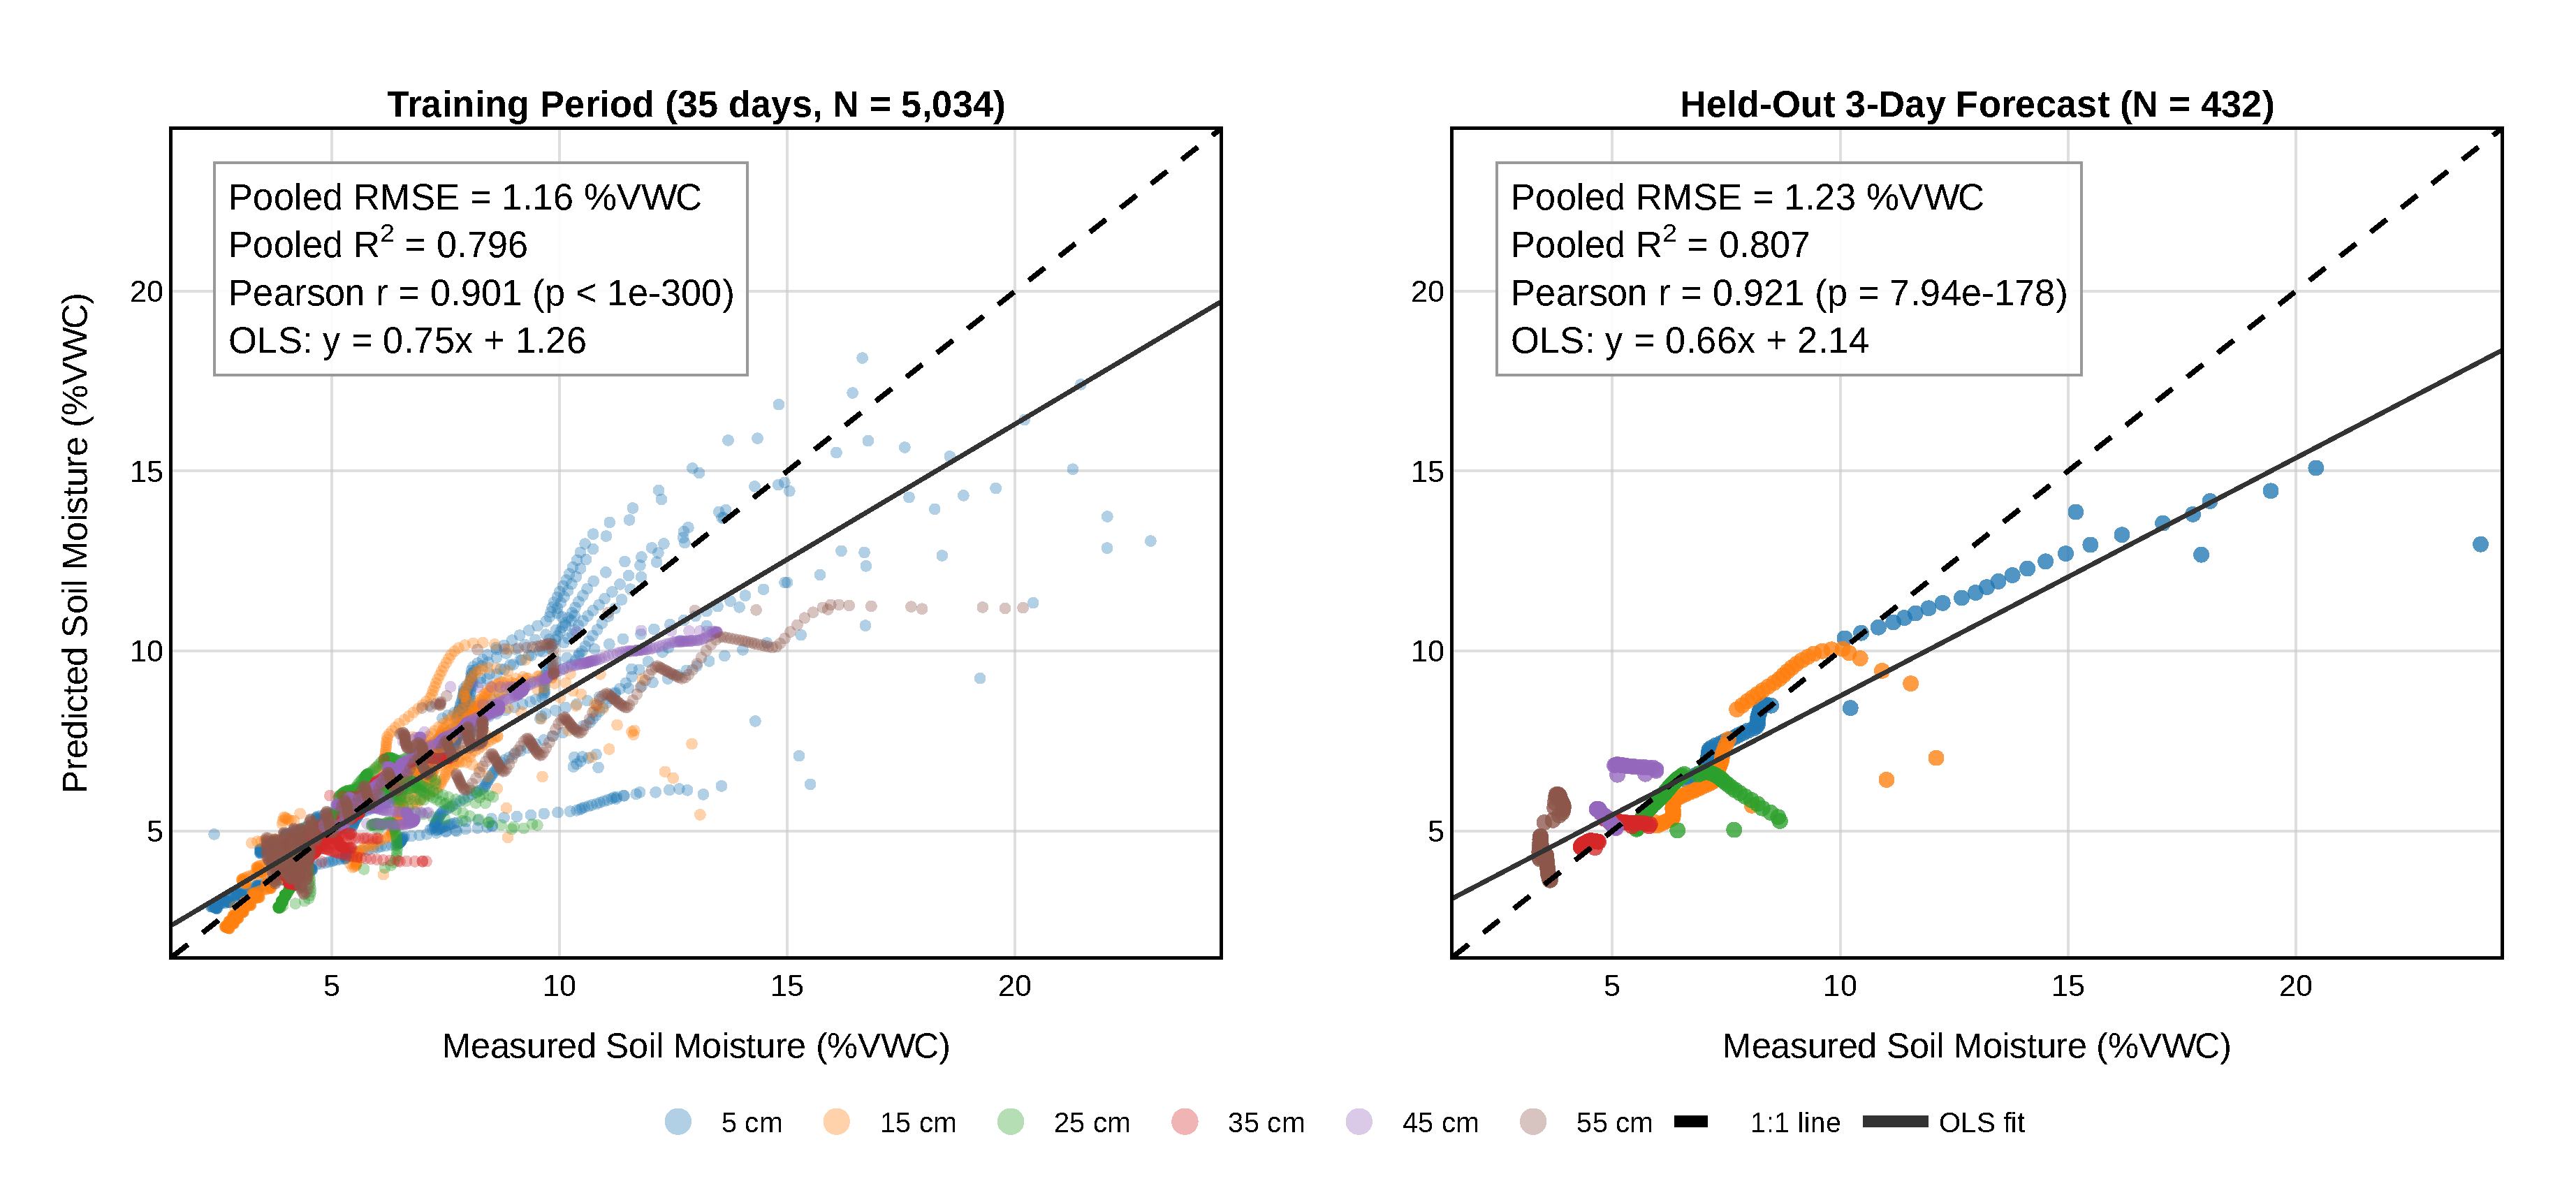
\includegraphics[width=0.96\linewidth]{predicted_vs_measured_scatter.pdf}
\caption{Predicted versus measured soil moisture parity scatterplots across all six sensor depths (5--55~\si{cm}) for the 35-day training period ($N = 5{,}034$ concatenated depth--hour points) and the 3-day held-out forecast ($N = 432$ points), illustrating tight clustering around the 1:1 line for low-variance deep layers (45--55~\si{cm}) alongside the profile-wide vertical span underlying the pooled $R^2 = 0.807$ and Pearson $r = 0.921$. Dashed lines denote the 1:1 parity reference, and solid lines show the ordinary least squares (OLS) linear regression fit.}
\label{fig:scatter_parity}
\end{figure}

In Fig.~\ref{errorfig}, the estimation error is distributed around zero during training and forecasting, where the box plots show that most of the error is distributed around zero (with interquartile ranges below \SI{2.5}{\%VWC}), along with some outliers due to the conservative behavior of the proposed PINN. Error peaks are evident at 5 \si{cm} and 55 \si{cm}; the peaks at 5 \si{cm} are correlated with rain and irrigation events, while the peaks at 55 \si{cm} are correlated with high rain events. The direct influence of rain at deeper layers is related to the terrain configuration, which consists of beds with lateral ditches that collect and drain excess water.

\begin{figure}[!htbp]
    \centering
    \includegraphics[width=\linewidth]{pinn_functions_vertical_by_layer.pdf}
    \caption{Estimated flux branches describing soil-water dynamics across sensor depths (5--55~\si{cm}, labeled along the left margin): $fr_i(r)$ is direct rainfall infiltration (\si{\%VWC/h}); $f_i(m_i)$ is gravitational vertical outflow (\si{\%VWC/h}); $f_{i,i+1}(m_i,m_{i+1})$ is signed potential-driven inter-layer exchange (\si{\%VWC/h}); $S_i(m_i,ET_0)$ is evapotranspirative depletion (\si{\%VWC/h}); $fl_i(m_i)$ is lateral ditch outflow (\si{\%VWC/h}, with scientific y-axis notation for compactness); and $fq_{\mathrm{irr}}(q_{\mathrm{irr}})$ is surface sprinkler inflow (\si{\%VWC/h}). Light blue regions denote the measured training moisture bounds at each depth.}
    \label{estimatedflows}
\end{figure}

The most relevant result is that the PINN approach offers interpretable information for control design or direct decision-making. Fig.~\ref{estimatedflows} illustrates the estimated functions of measurable variables describing the soil water dynamics, such as rain, soil moisture, $ET_0$, and irrigation. These estimated flows constitute the PINN as differential equations that accomplish water balances at each soil layer.
In the estimated functions, it is possible to observe that at the upper layer (5 \si{cm}), there is a linear relation between rain and soil moisture, where 30 \si{mm/h} of rain can induce an increase of 6 \si{\%VWC/h} in the soil moisture, and that in the third layer the direct increase is only 0.4 \si{\%VWC/h}. Moreover, it is observed that in the upper layer, 40 \si{\%VWC} induces vertical water movement that changes soil moisture by 3 \si{\%VWC/h}.

Furthermore, the estimated water movement associated with the potential difference between two soil layers is interlayer flow ($f_{i,i+1}$), ranging from $-6$ \si{\%VWC/h} (dark blue, upstream) to 3 \si{\%VWC/h} (yellow, downstream). It is noted that flows are generally consistent with potential gradients but are often negligible, consistent with sandy soil hydraulic properties \cite{Reyes2016}. The observed hydraulic trends between layers 1 and 2 can be attributed to changes in the soil induced by organic matter and agricultural practices.
The estimated evapotranspirative depletion ($S_i$, or $pc_i$) as a function of soil moisture and $ET_0$ increases with both. It is highlighted that layer 3 (25 \si{cm}) shows the maximum potential within the upper root zone to produce high moisture extraction, where at maxima of $ET_0$ and soil moisture, the produced change in soil moisture can be around 0.8 \si{\%VWC/h}, corroborating the proposed PINN as a tool to estimate soil regions where water must be guaranteed.
The estimated lateral outflow ($fl_i$) does not appear to be relevant for direct comparisons with the vertical movement of water. A particular small negative, non-monotonic behavior (despite the included constraints) appears in layer 5 ($fl_5(m_5)$) and reflects both lateral inflows from an adjacent ditch during storm surges and the fact that penalty terms $c_1$--$c_3$ act as finite soft regularizers rather than hard algebraic barriers.
Finally, it is estimated how irrigation ($fq_{\mathrm{irr}}(q_{\mathrm{irr}})$) increases the soil moisture. In this case, irrigation is considered in the surface layer because the field used sprinkler irrigation; however, the PINN configuration can be adjusted to the selected irrigation system by setting this inflow to the layer where it is applied. The estimated function is predominantly linear, where soil moisture in the surface layer increases by approximately 5 \si{\%VWC/h} per hour of irrigation. This is crucial for control and decision-making processes. For instance, this curve enables us to quickly determine the irrigation required to bring a crop from a measured soil moisture level to a desired point that ensures adequate water uptake in the surface layers, which is crucial during the early stages of perennial crops.
The shaded blue regions highlight the span of measured soil moisture data used for training, making evident the benefits and effects of the soft physical regularizers in the formulated approach, where, from sparse data, some functions like the vertical flow and lateral flow are reconstructed from the origin to far values following the positivity, monotonicity, and zero-forcing zero-flow regularizers.

\subsection{Benchmark Comparison, Ablation Study, and Control-Oriented Admissibility}\label{sec:benchmarks}

To evaluate whether the branched PINN topology, physical regularizers ($c_1$--$c_3$), and two-stage RK4 identification justify their complexity relative to simpler baselines, we compared eight closed-loop configurations using the identical hourly RK4 integrator ($\Delta t = \SI{1}{h}$): (1) the proposed \textbf{Full PINN} (375,089 parameters); (2) \textbf{Persistence} ($0$ parameters, $\hat{m}(t) = m(0)$); (3) a \textbf{Linear State-Space ODE} ($\dot{m} = Am + Bu + c_0$, 60 parameters fitted by ordinary least squares to Stage-1 finite differences); (4)--(6) unconstrained \textbf{Black-Box Neural ODEs} ($\dot{m} = \mathrm{MLP}(m, q_{\mathrm{irr}}, r, ET_0)$, four \texttt{mish} hidden layers), evaluated at capacity-matched width (\textbf{BlackBox-374k}, 374,156 parameters, Stage~1 only and Stage~1+2) and low-capacity width (\textbf{BlackBox-2.2k}, 2,190 parameters, Stage~1+2); (7) \textbf{Ablation~1 (PINN Stage~1 Only)}, omitting Stage-2 RK4 trajectory refinement ($j_2$); and (8) \textbf{Ablation~2 (PINN No Physics)}, trained with $\lambda_{c_1} = \lambda_{c_2} = \lambda_{c_3} = 0$. Aligning with the 3-day operational weather-forecast horizon, models were evaluated on the 35-day training period, the held-out 3-day benchmark, 30 rolling 3-day unseen windows (24-h stride across May~3--June~5, 2025, including storms with $r > \SI{25}{mm/h}$ and $ET_0 > \SI{0.73}{mm/h}$), and a 7-day (168~h) horizon sensitivity check (Table~\ref{tab:benchmarks_master}), alongside Jacobian physical admissibility audits (Table~\ref{tab:admissibility_audit}).

\begin{table}[!htbp]
\centering
\caption{Closed-loop forecasting benchmark and ablation study across all eight configurations over the 35-day training period, 3-day held-out forecast (pooled and 5-\si{cm} topsoil), 30 rolling 3-day unseen windows, and 7-day unseen rollout (\si{\%VWC}).}
\label{tab:benchmarks_master}
\fontsize{6.2}{7.8}\selectfont
\setlength{\tabcolsep}{1.6pt}
\begin{tabular*}{\textwidth}{@{\extracolsep{\fill}}lccccccc@{}}
\toprule
Model & Params & Train 35d & Held-Out 3d & 3d 5\,\si{cm} & \multicolumn{2}{c}{30 Rolling 3d Win.} & 7d Unseen \\
\cmidrule(lr){6-7}
 & & RMSE ($R^2$) & RMSE ($R^2$) & RMSE & Mean (SD) & Worst & RMSE ($R^2$) \\
\midrule
\textbf{Proposed PINN (Full)} & 375,089 & 1.16 (0.796) & 1.23 (0.807) & 2.02 & 1.04 (0.53) & 3.01 & 1.32 (0.705) \\
B1: Persistence & 0 & 2.44 (0.094) & 1.91 (0.539) & 4.32 & 1.86 (1.02) & 5.76 & 1.56 (0.588) \\
B2: Linear ODE & 60 & 1.35 (0.723) & 0.97 (0.880) & 1.71 & 0.82 (0.27) & 1.40 & 1.01 (0.829) \\
B3a: BB-374k (S1) & 374,156 & 2.93 ($-0.311$) & 1.02 (0.868) & 1.98 & 0.86 (0.40) & 2.39 & 0.83 (0.884) \\
B3b: BB-374k (S1+2) & 374,156 & 0.91 (0.874) & 1.13 (0.838) & 1.73 & 0.98 (0.57) & 2.90 & 1.45 (0.644) \\
B3c: BB-2.2k (S1+2) & 2,190 & 0.85 (0.890) & 1.26 (0.797) & 1.66 & 1.77 (2.43) & 11.41 & 1.98 (0.337) \\
Abl.1: PINN (S1 only) & 375,089 & 2.52 (0.032) & 1.55 (0.696) & 2.65 & 1.33 (0.35) & 2.43 & 1.87 (0.412) \\
Abl.2: PINN ($\lambda_c{=}0$) & 375,089 & 1.48 (0.665) & 1.39 (0.756) & 2.89 & 1.00 (0.30) & 1.77 & 1.46 (0.641) \\
\bottomrule
\end{tabular*}
\begin{tablenotes}
\footnotesize
\item Note: Across 14 extreme forcing windows ($r > 25\,\si{mm/h}$ or $ET_0 > 0.73\,\si{mm/h}$), mean 3-day RMSE is \SI{1.04}{\%VWC} for Proposed PINN versus \SI{1.95}{\%VWC} for Persistence, \SI{1.97}{\%VWC} for BB-2.2k (S1+2), and \SI{1.26}{\%VWC} for Ablation~1. Over extended 14-day unassisted rollouts, RMSE ($R^2$) is 1.74 (0.391) for Proposed PINN versus 2.14 (0.079) for BB-374k (S1+2), 2.99 ($-0.800$) for BB-2.2k (S1+2), and 2.22 (0.002) for Ablation~1.
\end{tablenotes}
\end{table}

Table~\ref{tab:benchmarks_master} confirms the role of each PINN component. Relative to Persistence, the Full PINN reduces held-out 3-day RMSE by 35.6\% (1.91 to 1.23~\si{\%VWC}), cuts dynamic 5-\si{cm} topsoil RMSE by 53.2\% (4.32 to 2.02~\si{\%VWC}), lowers 30-window mean RMSE from 1.86 to 1.04~\si{\%VWC} (extreme-storm windows: 1.95 to 1.04~\si{\%VWC}), and nearly halves worst-window error (5.76 to 3.01~\si{\%VWC}). Omitting Stage-2 RK4 refinement (Ablation~1) degrades every horizon—worsening 35-day training RMSE from 1.16 to 2.52~\si{\%VWC} ($R^2 = 0.032$), 3-day forecast RMSE to 1.55~\si{\%VWC}, 30-window mean to 1.33~\si{\%VWC}, and 7-day RMSE to 1.87~\si{\%VWC}—confirming that Stage-2 output-error matching eliminates cumulative integration drift. Removing physical regularizers (Ablation~2, $\lambda_c = 0$) degrades training (1.48~\si{\%VWC}), 3-day forecasting (1.39~\si{\%VWC}; 5-\si{cm} topsoil rising from 2.02 to 2.89~\si{\%VWC}), and 7-day rollout (1.46~\si{\%VWC}) while inducing severe internal constraint violations (Table~\ref{tab:admissibility_audit}). Meanwhile, the low-capacity unconstrained BlackBox-2.2k overfits the training trajectory (0.85~\si{\%VWC}) yet generalizes poorly across the 30 unseen 3-day windows (mean 1.77~\si{\%VWC}, worst 11.41~\si{\%VWC}) and 7-day horizon (1.98~\si{\%VWC}).

Crucially, comparing Tables~\ref{tab:benchmarks_master} and \ref{tab:admissibility_audit} highlights a fundamental distinction between passive trajectory interpolation and control-admissible identification. Under passive historical replay, the unconstrained Linear ODE (0.97~\si{\%VWC}) and overparameterized BlackBox-374k (1.02--1.13~\si{\%VWC}) achieve slightly lower aggregate 3-day RMSE (by 0.10--0.26~\si{\%VWC}, i.e., $\approx 0.1$--$0.26\,\si{mm}$ per layer) by exploiting non-causal cross-depth correlations on quasi-static deep horizons, although BlackBox-374k (S1+2) degrades faster than the PINN at 7 days (1.45 vs.\ 1.32~\si{\%VWC}) and 14 days (2.14 vs.\ 1.74~\si{\%VWC}), and BlackBox-374k (S1) produces unphysical negative moisture ($\hat{m}_i < 0$) on 9.59\% of unclipped multi-week rollout steps. More importantly, automatic-differentiation Jacobian audits across observed unseen trajectories ($N = 792$~h) and 2,000 uniform domain states in $[0,1]^9$ (Table~\ref{tab:admissibility_audit}) show that \emph{every unconstrained baseline violates physical actuation signs}: BlackBox-374k (S1+2) and BlackBox-2.2k (S1+2) exhibit negative topsoil irrigation gain ($\partial \dot{m}_1/\partial q_{\mathrm{irr}} < 0$) at 52.90\% and 96.84\% of trajectory states, respectively, and positive moisture sensitivity to evapotranspiration ($\partial \dot{m}_i/\partial ET_0 > 0$) at 40.74\% and 28.24\% of states, while the Linear ODE exhibits permanent 33.33\% structural sign inversions for both $q_{\mathrm{irr}}$ and $ET_0$ alongside dry-state suction ($-0.652\,\si{\%VWC/h}$). Embedded inside an MPC optimizer, such sign inversions can prescribe less irrigation to wet the soil or predict wetting under high evaporative demand. By contrast, the Full PINN achieves \textbf{0.00\%} irrigation-gain sign inversions ($\min \partial \dot{m}_1/\partial q_{\mathrm{irr}} = +3.99\,\si{\%VWC/h}$ per \si{h/h}), \textbf{0.00\%} negative rainfall slopes, \textbf{0.00\%} unclipped negative states, minimal residual $\partial \dot{m}_i/\partial ET_0 > 0$ (2.05\%/2.46\%, $\max = 0.020\,\si{\%VWC/h}$ vs.\ $2.72$--$5.80$ in black-box models), and near-zero internal violations ($0.004\%$ $c_1$, $0.34\%$ $c_2$ vs.\ $26.67\% / 19.51\%$ when $\lambda_c=0$).

\begin{table}[!htbp]
\centering
\caption{Control-oriented Jacobian admissibility and internal constraint audit across the $[0,1]^9$ domain ($2{,}000$ samples) and unseen trajectory states ($N = 792$~h), alongside unclipped negative state rate and dry zero-input drift ($\dot{m}$ at $m=0, u=0$).}
\label{tab:admissibility_audit}
\fontsize{6.2}{7.8}\selectfont
\setlength{\tabcolsep}{0.9pt}
\begin{tabular*}{\textwidth}{@{\extracolsep{\fill}}lcccccccc@{}}
\toprule
Model & Unclip. & \multicolumn{2}{c}{$\partial_{q_{\mathrm{irr}}}\dot{m}<0$ (\%)} & Dom.\,$\partial_r\dot{m}{<}0$ & \multicolumn{2}{c}{$\partial_{ET_0}\dot{m}>0$ (\%)} & ZeroEq & Internal \\
\cmidrule(lr){3-4}\cmidrule(lr){6-7}
 & $<0$ (\%) & Traj.\,$\dot{m}_1$ & Dom.\,all & (\%) & Traj. & Dom. & ($+/-$) & $c_1 / c_2$ (\%) \\
\midrule
\textbf{Proposed PINN (Full)} & \textbf{0.00} & \textbf{0.00} & \textbf{0.00} & \textbf{0.00} & 2.46 & 2.05 & $+0.074/0.000$ & \textbf{0.004 / 0.34} \\
B1: Persistence & 0.00 & 0.00 & 0.00 & 0.00 & 0.00 & 0.00 & $0.000/0.000$ & --- \\
B2: Linear ODE & 0.00 & 0.00 & 33.33 & 0.00 & 33.33 & 33.33 & $+0.256/-0.104$ & --- \\
B3a: BB-374k (S1) & 9.59 & 68.94 & 35.36 & 10.23 & 19.17 & 31.55 & $+0.293/-0.132$ & --- \\
B3b: BB-374k (S1+2) & 0.00 & 52.90 & 48.50 & 10.32 & 40.74 & 30.58 & $+0.317/-0.191$ & --- \\
B3c: BB-2.2k (S1+2) & 0.00 & 96.84 & 39.78 & 17.41 & 28.24 & 28.58 & $+0.252/+0.042$ & --- \\
Abl.1: PINN (S1 only) & 0.00 & 0.00 & 0.00 & 0.00 & 0.99 & 0.44 & $+0.038/0.000$ & 0.00 / 0.14 \\
Abl.2: PINN ($\lambda_c{=}0$) & 0.00 & 0.00 & 0.00 & 6.12 & 41.98 & 17.57 & $0.000/-0.055$ & 26.67 / 19.51 \\
\bottomrule
\end{tabular*}
\begin{tablenotes}
\footnotesize
\item Note: Domain minimum topsoil irrigation gain $\min(\partial \dot{m}_1/\partial q_{\mathrm{irr}})$ is $+3.99\,\si{\%VWC/h}$ per \si{h/h} for Proposed PINN versus $-22.99$, $-22.21$, and $-23.16$ for BB-374k (S1), BB-374k (S1+2), and BB-2.2k (S1+2). Domain maximum $\partial \dot{m}_i/\partial ET_0$ is $0.020\,\si{\%VWC/h}$ per \si{mm/h} for Proposed PINN versus $2.87$, $2.72$, and $5.80$ for the three black-box baselines.
\end{tablenotes}
\end{table}

\subsection{Agronomic and Hydrological Interpretation of Inferred Evapotranspirative Depletion}\label{sec:uptake_rationale}

Because the sink branch $S_i(m_i, ET_0)$ ($pc_i$ in Fig.~\ref{Mainfig}) is identified solely from volumetric moisture dynamics and $ET_0$, it represents an \emph{apparent $ET_0$-correlated layer moisture depletion rate} rather than isolated plant transpiration, aggregating three radiation-in-phase processes~\cite{Feddes1978, allen1998crop}: (i) surface soil evaporation at 5~\si{cm}; (ii) shallow root-water uptake; and (iii) diurnal capillary drawdown and ditch-bank evaporation coupled to adjacent drainage ditches.

Daily integration of $\sum_{i=1}^{6} pc_i$ across complete 24-h days yields physically realistic magnitudes: \SI{2.04}{mm/d} in training ($n = 34$ days, IQR $[1.89, 2.46]$, range $[0.43, 2.88]\,\si{mm/d}$, mean $ET_0 = \SI{4.12}{mm/d}$, ratio $0.50$) and \SI{1.89}{mm/d} across the unseen validation season ($n = 32$ days, IQR $[1.53, 2.39]$, range $[0.46, 3.00]\,\si{mm/d}$, mean $ET_0 = \SI{3.85}{mm/d}$, ratio $0.49$), consistent with spring Florida Flatwoods citrus evapotranspiration ($\approx 2$--$5\,\si{mm/d}$, reduced under HLB canopy stress and localized micro-sprinkler wetting)~\cite{Morgan2006, Castle1993, allen1998crop}. Vertically, the upper root zone (5--25~\si{cm}) accounts for \SI{0.58}{mm/d} (28.5\%: \SI{0.22}{mm/d} [10.9\%] at 5~\si{cm}, \SI{0.08}{mm/d} [3.8\%] at 15~\si{cm}, and an upper-root maximum of \SI{0.28}{mm/d} [13.8\%] at 25~\si{cm} directly above the $\approx\SI{30}{cm}$ argillic clay hardpan~\cite{Morgan2006, Castle1993}), mid-depth clay horizons extract \SI{0.05}{mm/d} (2.4\% at 35~\si{cm}) and \SI{0.11}{mm/d} (5.5\% at 45~\si{cm}), and the 55-\si{cm} layer accounts for \SI{1.30}{mm/d} (63.5\%) due to daytime water-table and ditch-level recession at the raised-bed base rather than deep rooting below the hardpan (Fig.~\ref{fig:bed_ditch}). Partitioning physiological transpiration from soil evaporation and ditch exchange would require independent sap-flow or lysimetry sensors beyond the scope of this study.

\subsection{Conclusions}
Accurate forecasting of multi-depth soil moisture dynamics has been constrained by analytical Richards' equation solvers requiring intensive site-specific hydraulic calibration and by unconstrained black-box models that violate control-admissibility requirements. Here, we show that embedding a sensor-depth finite-volume discretization of Richards' equation into a physically regularized two-stage PINN reconciles flux-level interpretability with operational multi-day forecasting accuracy.

Validated on field telemetry from a commercial raised-bed Florida citrus block, the closed-loop PINN predicts hourly soil moisture across six depths (5--55~\si{cm}) over a 3-day held-out horizon with a pooled RMSE of \SI{1.23}{\%VWC} (\SI{3.22}{mm} over the 60-\si{cm} profile, $R^2 = 0.807$, Pearson $r = 0.921$), reduces 3-day error by 35.6\% relative to persistence, outperforms single-stage and unregularized ablations across 30 rolling 3-day unseen windows and a 7-day rollout, and eliminates the 33\%--97\% control-sign inversions exhibited by unconstrained linear and black-box Neural ODE baselines while exposing explicit irrigation gain and evapotranspirative depletion curves.

Key scope boundaries merit emphasis. First, calibration and validation were conducted at a single raised-bed sandy Alfisol citrus grove across a 35-day training period and 33-day spring unseen dataset using observed station forcing on held-out horizons; generalization to finer-textured soils, other crops, and live scheduling under noisy numerical weather forecasts requires multi-site, multi-season evaluation. Second, hourly sampling imposed by forecast providers smooths sub-hourly infiltration peaks in sandy topsoil. Finally, while the PINN satisfies structural and Jacobian conditions suitable for model predictive control (MPC), closed-loop field MPC deployment and direct measurement of irrigation water savings remain essential future work rather than demonstrated outcomes of this study.


\section{Methodology: PINN Formulation} \label{Methodology}
\subsection{Problem Statement}
We address the formulation of a model suitable for precise decision-making in irrigation management. The model's precision is primarily focused on vertical water distribution, where, in a horizontally homogeneous soil region, soil moisture measurements from a particular section can be considered significant for making informed irrigation decisions. This practice is common in most commercial settings where irrigation is managed using soil moisture sensors \cite{Rossini2021, Mandal2025}.
Therefore, the model must accurately describe the vertical dynamics of soil moisture and their interaction with evapotranspirative plant-soil sink processes, environmental variables, and irrigation. Specifically, the model must describe the soil moisture dynamics at the targeted measured soil layers $m_i(t)$ (\si{\%VWC}). 
Moreover, at each layer, the model must explain the effects of measurable external inputs, such as rainfall $r(t)$ (\si{mm/h}), irrigation rate $q_{\mathrm{irr}}(t)$ (\si{h/h}), and potential evapotranspiration $ET_0(t)$ (\si{mm/h}), which drives root-zone water depletion.
In addition, the model must be interpretable, physically consistent, and stable, mirroring the stability observed in the real system under unsaturated conditions.
Importantly, the model must allow the incorporation of valuable forecast information in its numerical simulation over extended horizons to support the formulation of model predictive control (MPC) frameworks.


\subsection{Proposed Approach}

Figure \ref{diagramalgorithm} describes the proposed PINN architecture and training process. The architecture comprises an input layer associated with variables that can be obtained from field sensors, estimated, or obtained from forecasting services; therefore, the measured soil moisture initial condition ($m(0)$), measured irrigation, measured evapotranspiration, measured rainfall, and the current estimated soil moisture ($\hat{m}(t)$) are considered as inputs.

The hidden layers are designed to match the structure of a spatially discretized Richards' equation, with $n$ vertical layers corresponding to the depths of installed soil moisture sensors in the field. These layers are configured as fluxes that are functions of the measured and estimated variables. These fluxes represent elements of Richards' equation, such as gravitational drainage and capillary-driven water movement. Moreover, these fluxes include inflow from rainfall and irrigation and incorporate plant water uptake as a function of $ET_0$ and soil moisture. Therefore, the fluxes in the hidden layers are modeled by neural networks with parameters $\Theta$ that form the dynamic model, a set of differential equations describing the temporal variation of soil moisture in each layer. This set of differential equations is numerically solved using a 4th-order Runge–Kutta (RK4) algorithm, which is integrated directly into the training and implementation routines.

The training process searches for the $\Theta$ parameters that promote an accurate description of the SM dynamics of the real system. The training process utilizes recorded windows of training data. The integration of the RK4 routine into the training process ensures a solution that, starting from a measured initial soil moisture condition $m(0)$, uses rainfall, potential evapotranspiration, and irrigation data to provide an optimal or near-optimal description of soil moisture dynamics. This inclusion contributes to model stability and generality. However, including numerical integration of the model in the training process significantly complicates the optimization problem. Therefore, the training is conducted in two stages. The first stage minimizes the derivative losses between measured and estimated soil moisture variations; this routine does not require numerical integration and is a strategy for finding a point to initialize the $\Theta$ parameters near a feasible solution. The second stage employs the tracking loss, which embeds the model's numerical solution to align the estimated SM ($\hat{m}(t)$) with the measured SM ($m(t)$).
Furthermore, the cost function incorporates three penalization conditions: positivity ensures the correct flow direction in the discretized Richards' equation, monotonicity guarantees flow correlation with driving variables, and zero-potential zero-flux enforces the absence of flow when no water source is present.
Ultimately, a trained model with its respective numerical solver is obtained. This model allows the inclusion of external inputs, such as rainfall and $ET_0$, which can be obtained directly or inferred from forecasting services. Importantly, the model is also a function of the irrigation (the control input), which can be obtained using predictive control approaches or used to evaluate multiple irrigation scenarios. Moreover, including water uptake, treated as a function of $ET_0$ and soil moisture, in the overall model enables inference of the amount of water correlated with plant water uptake, helping dynamically identify and prioritize regions where the estimated plant is absorbing the most water.
Subsequently, a detailed description of the model's modeling, formulation, training, and implementation in a real citrus field is provided.

\begin{figure}[!htbp]
		\centering
		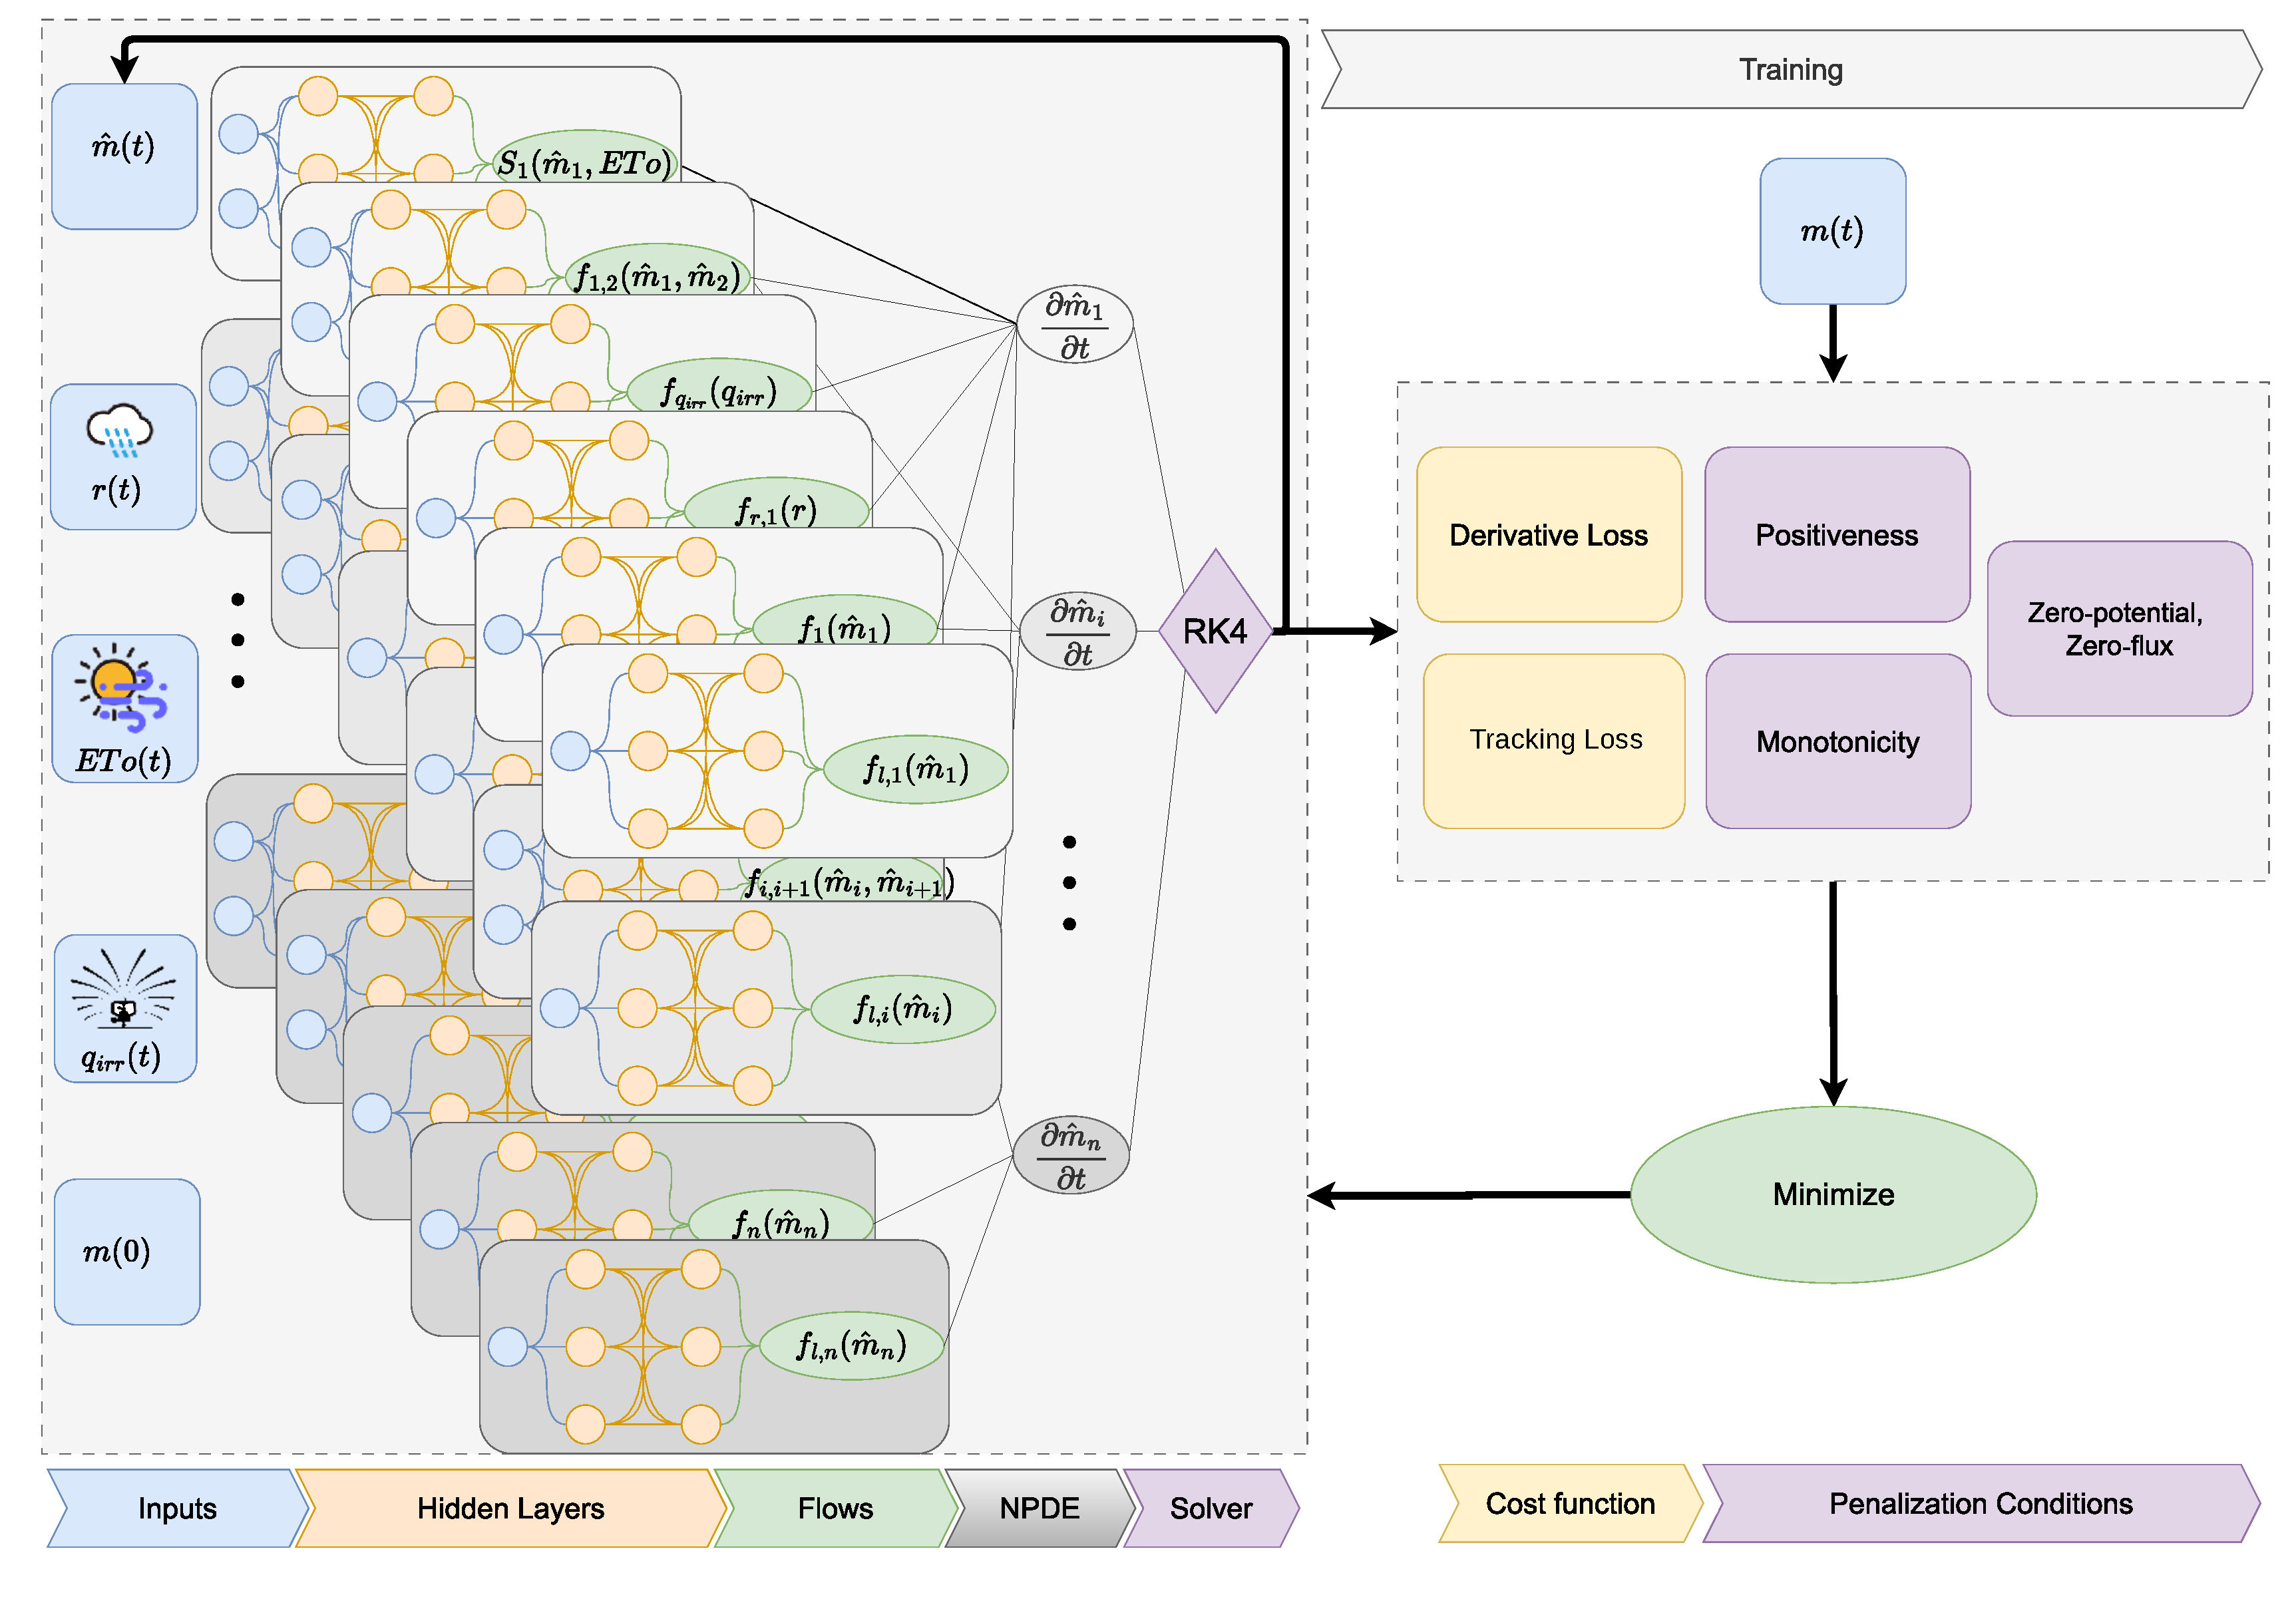
\includegraphics[width=0.92\textwidth]{PINNsmb.pdf}
		\caption{Architecture and two-stage training workflow of the proposed PINN. Inputs comprise the 6-layer moisture vector $\hat{m}(t)$ (5--55~\si{cm}), irrigation ($q_{\mathrm{irr}}$), rainfall ($r$), and reference evapotranspiration ($ET_0$). Inside $g(\hat{m},r,ET_0,q_{\mathrm{irr}},\boldsymbol{\Theta})$, neural branches model vertical drainage $f_i(m_i)$, signed inter-layer exchange $f_{i,i+1}(m_i,m_{i+1})$ ($i=1\dots5$), lateral ditch outflow $fl_i(m_i)$ ($i=1\dots5$; $f_6$ captures lower boundary discharge), rainfall infiltration $fr_i(r)$, surface irrigation $fq_{\mathrm{irr}}(q_{\mathrm{irr}})$, and evapotranspirative sink $S_i(m_i,ET_0)$ ($pc_i$). Stage~1 minimizes derivative loss $j_1$ and Stage~2 refines $\boldsymbol{\Theta}$ via RK4 trajectory tracking loss $j_2$, subject to soft penalties $c_1$--$c_3$.}
		\label{diagramalgorithm}
  \vspace{-1em}
\end{figure}

\subsubsection{Model}\label{sec2}

The developed Physics-Informed Neural Network (PINN) is formulated using a spatial discretization of Richards' equation, which describes vertical water movement in the soil as a function of soil moisture. We propose a spatial discretization by dividing the soil into $n$ layers, with each layer associated with available soil moisture measurements. The objective is to determine the rate of change of soil moisture in each layer due to gravity and water potential. Let $z$ denote the vertical depth coordinate taken positive downward, and let $H = h(m) - z$ denote total hydraulic head, where $h(m)$ is the soil-water matric pressure head and $-z$ is gravitational potential relative to the soil surface. By the Darcy--Buckingham law, the downward vertical water flux $q$ (positive downward) is:
\begin{equation}
q = -K(m)\frac{\partial H}{\partial z} = -K(m)\left(\frac{\partial h(m)}{\partial z} - 1\right) = K(m)\left(1 - \frac{\partial h(m)}{\partial z}\right),
\label{eq:darcy}
\end{equation}
where $K(m)$ is the moisture-dependent hydraulic conductivity. Substituting Eq.~\eqref{eq:darcy} into the 1D mass-continuity conservation law,
\begin{equation}
\frac{\partial m}{\partial t} = -\frac{\partial q}{\partial z},
\label{continuity}
\end{equation}
yields Richards' equation for downward-positive depth $z$:
\begin{equation}
\frac{\partial m}{\partial t} = \frac{\partial }{\partial z}\left[ K(m)\left(\frac{\partial h(m)}{\partial z} - 1\right)\right].
\label{Richards}
\end{equation}
Using forward finite-volume discretization along $z$ with uniform compartment thickness $\Delta z$, evaluating $\partial h/\partial z \approx (h(m_{i+1}) - h(m_i))/\Delta z$ across the lower interface between layers $i$ and $i+1$, the downward flux $q_i$ leaving layer $i$ into layer $i+1$ is:
\begin{equation}
q_i = K(m_i)\left(\frac{h(m_i)-h(m_{i+1})}{\Delta z}+1\right).
\label{eq:flux_disc}
\end{equation}
Similarly, the continuity equation describing moisture conservation in layer $i$ is discretized as:
\begin{equation}
\frac{d m_i}{d t} = \frac{q_{i-1}(t)-q_i(t)}{\Delta z}.
\label{eq:cont_disc}
\end{equation}
Boundary conditions close the 1D vertical column at the soil surface ($i=1$) and lower profile boundary ($i=n$): the upper boundary receives effective surface inflow $q_0(t)$ supplied by rainfall and sprinkler irrigation minus surface evaporative losses, while the bottom boundary ($z = 60\,\si{cm}$) discharges vertically via $f_n(m_n)$ without a separate lateral ditch-outflow branch.

Substituting Eq.~\eqref{eq:flux_disc} into Eq.~\eqref{eq:cont_disc} provides the discretized vertical balance at interior layer $i$:
\begin{equation}
\begin{aligned}
\frac{d m_i}{d t} &= K(m_{i-1})\left(\frac{h(m_{i-1})-h(m_{i})}{\Delta z^2}\right) + \frac{K(m_{i-1})}{\Delta z} \\
&\quad - K(m_{i})\left(\frac{h(m_{i})-h(m_{i+1})}{\Delta z^2}\right) - \frac{K(m_{i})}{\Delta z}.
\end{aligned}
\label{eq:disc_richards}
\end{equation}
From this discretized formulation, it can be observed that the rate of change of soil moisture at each $i$-th layer, driven by gravity and matric potential gradients, can be parameterized by neural sub-functions of measured soil moisture in the respective and adjacent layers:
\begin{equation}
\begin{aligned}
K(m_{i})\left(\frac{h(m_{i})-h(m_{i+1})}{\Delta z^2}\right) &\approx f_{i,i+1}({m}_i,{m}_{i+1}), \\ 
\frac{K(m_{i})}{\Delta z} &\approx f_i({m}_i),
\end{aligned}
\end{equation}
where $f_i(m_i) \ge 0$ captures downward gravitational drainage and $f_{i,i+1}(m_i, m_{i+1})$ captures potential-driven inter-layer redistribution, which is intentionally left signed (positive downward when $m_i > m_{i+1}$, negative for upward capillary rise when $m_{i+1} > m_i$).

Moreover, additional functions describing the rate of change produced by actions such as irrigation, rainfall, water uptake, and horizontal water movement can be incorporated to obtain a model structure that could be useful for evaluating how soil moisture dynamics evolve over time in response to external variables. Specifically, $q_{\mathrm{irr}}$ is incorporated as the irrigation-related variable, and $fq_{\mathrm{irr}}(q_{\mathrm{irr}})$ is a function that explains the rate of change of the soil moisture in relation to irrigation. Note that $q_{\mathrm{irr}}$ can be expressed either in volumetric flow units (e.g., \si{m^3/h}) or in relative irrigation-duration units (\si{h/h}), indicating the fraction of the sampling hour during which irrigation was active (used in this field study). In the first case, $fq_{\mathrm{irr}}(q_{\mathrm{irr}})$ provides a relation between applied flow and change in soil moisture, and in the second case, $fq_{\mathrm{irr}}(q_{\mathrm{irr}})$ provides a relation between duration of irrigation time and change in soil moisture. In this study, we assume that irrigation is applied only at the top, but its location can be accommodated depending on the irrigation system used, e.g., subsurface drip irrigation. 
The rainfall, $r$, is considered an input in \si{mm/h} and can be obtained from a weather station in the crop or from meteorological services, where predictions are also available. The function, $fr_i(r)$, accounts for the direct effect of rain at each soil layer. This is because crops are often planted in beds, allowing rain to wet exposed soil layers directly.

Furthermore, we incorporate a sink component to estimate soil moisture changes due to evapotranspirative depletion in each layer, which is a key motivation for this study. This sink is represented by an evapotranspirative sink function, $S_i (m_i, ET_0)$ (denoted $pc_i$ in Section~\ref{Results}), describing moisture depletion at each layer governed by atmospheric, plant, and soil conditions \cite{swap2024}. Specifically, we propose that this sink is a function of the available water at the respective layer ($m_i$) and the potential evapotranspiration ($ET_0$).
Additionally, we include an outlet lateral flow, $fl_i (m_i)$, associated with subsurface drainage toward adjacent ditches when excess water accumulates across layers. This is considered an outlet, as most crops are planted in raised beds between furrows or ditches to facilitate drainage.

In summary, we are formulating a PINN to estimate the dynamics of a system with $n$ soil layers ($n=6$) as follows:
\begin{equation}
\label{system}
\begin{aligned}
\frac{d{m}_1}{dt} = & - f_1({m}_1) - f_{1,2}({m}_1,{m}_2) - fl_1(m_1) - S_1({m}_1, ET_0) + fr_1(r) + fq_{\mathrm{irr}}(q_{\mathrm{irr}})\\
\frac{d{m}_i}{dt} = & f_{i-1}({m}_{i-1}) + f_{i-1,i}({m}_{i-1},{m}_i) - f_i({m}_i)- f_{i,i+1}({m}_i,{m}_{i+1}) - fl_i(m_i) \\ 
 & - S_i({m}_i, ET_0) + fr_i(r), \qquad i = 2,\dots,n-1,\\
\frac{d{m}_n}{dt} = & f_{n-1}({m}_{n-1}) + f_{n-1,n}({m}_{n-1},{m}_n) - f_n({m}_n) - S_n({m}_n, ET_0) + fr_n(r).
\end{aligned}
\end{equation}
Note that at layer $n$ ($n=6$, \SI{55}{cm}), we exclude the lateral flow term $fl_n$. In the upper layers, the vertical flow $f_i$ delivers water to the layer below, making it distinct from the lateral flow $fl_i$, which exits the system. However, at layer $n$, both $f_n$ and $fl_n$ would represent outflows that leave the soil column without feeding another layer, making them similar.

\subsubsection{PINN Structure}
In our approach, we use the system structure proposed in (Eq. \eqref{system}) to define the PINN structure. Therefore, as shown in Fig. \ref{diagramalgorithm}, we are proposing an NN with branches that emulate the functions \( g \in \{f_i, f_{i,i+1}, S_i, fq_{\mathrm{irr}}, fr_i, fl_i\} \). Therefore, each branch is a Multilayer Perceptron (MLP) with depth \( L \) and hidden width \( H_{\mathrm{b}} \), given by
\begin{equation}
\phi\!\bigl(\mathbf{x}; \boldsymbol{\Theta}\bigr)
  =\;
  \mathbf{W}^{(L)}
  \,\mathcal{A}\!\Bigl(
     \mathbf{W}^{(L-1)}
     \,\mathcal{A}\!\bigl(
        \dots
        \,\mathcal{A}\!\bigl(
           \mathbf{W}^{(1)}\mathbf{x}
           +\mathbf{b}^{(1)}
        \bigr)
        +\mathbf{b}^{(L-1)}
     \bigr)
  \Bigr)
  +\mathbf{b}^{(L)},
\label{eq:mlp}
\end{equation}
where \(\mathcal{A}(\cdot)\) is the activation function, and \(\displaystyle \boldsymbol{\Theta} = \{\mathbf{W}^{(\ell)},\,\mathbf{b}^{(\ell)}\}_{\ell=1}^L\) is the set of trainable parameters across branch depth \(L\) and hidden width \(H_{\mathrm{b}}\). Specifically, in the implemented architecture (\texttt{pinn\_model.py}): (i) non-negative single-input branches (\(f_1\dots f_5\), \(fq_{\mathrm{irr}}\), \(fr_1\dots fr_6\), and \(fl_1\dots fl_5\)) use \texttt{mish} activations with zero bias (\(\mathbf{b}^{(\ell)}=\mathbf{0}\)) and hidden width \(H_{\mathrm{b}}=H=56\) across three hidden layers (\(L=4\)); (ii) signed inter-layer exchange branches (\(f_{1,2}\dots f_{5,6}\)) and the lower boundary branch (\(f_6\)) use \texttt{tanh} activations (\(H_{\mathrm{b}}=H=56\), \(L=4\); zero bias on \(f_{i,i+1}\) and trainable bias on \(f_6\)) to accommodate bidirectional signed fluxes; and (iii) two-input evapotranspirative sink branches (\(S_1\dots S_6\)) use \texttt{mish} activations with zero bias and doubled hidden width \(H_{\mathrm{b}}=2H=112\) across four hidden layers (\(L=5\)). The input \(\mathbf{x}\) denotes the argument of each flux function.
In cases where the function depends on a single variable $\left(f_i(m_i),\;fq_{\mathrm{irr}}(q_{\mathrm{irr}}),\;fr_i(r),\;fl_i(m_i)\right)$, we have \(\mathbf{x}\in\mathbb{R}\), and when the function depends on two variables \(f_{i,i+1}(m_i,m_{i+1})\), \(\displaystyle \mathbf{x}=[m_i,m_{i+1}]^\top\in\mathbb{R}^2\); and for \(S_i(m_i,ET_0)\), \(\displaystyle \mathbf{x}=[m_i,ET_0]^\top\in\mathbb{R}^2\). Moreover, the dimensions of the first-layer weight matrices are \(\mathbf{W}^{(1)}\in\mathbb{R}^{H_{\mathrm{b}}\times1}\) for scalar inputs, and \(\mathbf{W}^{(1)}\in\mathbb{R}^{H_{\mathrm{b}}\times2}\) for two-dimensional inputs as encountered in \(f_{i,i+1}\) and \(S_i\).
\( \mathbf{W}^{(\ell)} \in \mathbb{R}^{H_{\mathrm{b}} \times H_{\mathrm{b}}} \) for \( \ell = 2, \dots, L-1 \), and \( \mathbf{W}^{(L)} \in \mathbb{R}^{1 \times H_{\mathrm{b}}} \). With biases \( \mathbf{b}^{(\ell)} \in \mathbb{R}^{H_{\mathrm{b}}} \) for \( \ell = 1, \dots, L-1 \), and \( \mathbf{b}^{(L)} \in \mathbb{R} \) (set to zero on all zero-origin branches and trainable on \(f_6\)), yielding an exact total of 375,089 trainable parameters across all 29 branches at \(H=56\).

Note that for brevity, a compact description of the system can be formulated as 

\begin{equation}
    \label{systemtheta}
    \dot{m}(t) = g(m,r,ET_0,q_{\mathrm{irr}},\boldsymbol{\Theta}).
\end{equation}


\subsubsection{Optimization Problem and Training}\label{subsec2}

As shown in the model formulation, PINN is a highly flexible technique that allows incorporating all physical and even empirical knowledge about the system into the PINN structure. Additionally, the formulation of the optimization problem provides an opportunity to shape the estimated system, including information that can contribute to model generalization and the estimated system's physical correctness. Therefore, the optimization problem is formulated to parameterize the system~\eqref{systemtheta}, aiming that this: i) mimics soil-water and evapotranspirative water depletion dynamics; ii) provides a clear explanation of the effects of the considered fluxes on the system; and iii) is useful for the design of control or decision-making approaches, especially predictive control approaches.

\subsubsection{Data Preparation for Training}

The approach uses a moving-horizon data window for training, enabling a model that can be periodically tuned using stored system measurements, consistent with the strategy presented in \cite{condeforecast2024, Alessandri2017}. To condition gradient-based optimization, all physical variables are normalized into \([0, 1]\) using fixed domain-scaling constants matched to operational field bounds: soil moisture by \SI{40}{\%VWC} (\(m_{\mathrm{scaled}} = m / 40\)), rainfall by \SI{30}{mm/h} (\(r_{\mathrm{scaled}} = r / 30\)), reference evapotranspiration by \SI{0.8}{mm/h} (\(ET_{0,\mathrm{scaled}} = ET_0 / 0.8\)), and irrigation duration fraction by \SI{1.0}{h/h} (\(q_{\mathrm{irr,scaled}} = q_{\mathrm{irr}} / 1\)), with hourly integration step \(\Delta t = \SI{1}{h}\). To clarify the estimation process, the following notation is introduced, where \( n_e \) is the size of the estimation window and \( t_k \) is the current time instant.

Let \( m(t_k) = [m_1(t_k), m_2(t_k), \dots, m_n(t_k)]^\top \in \mathbb{R}^{n} \) denote the measured soil moisture at $n$ depths ($n=6$) at the current time \( t_k \), and let \( m_i(t_{k_e \mid k}) \) denote the time series of measurements at depth \( i \) over an estimation window of size $n_e$, defined as  
${m_i(t_{k_e \mid k})}=\left[m_i(t_{k-n_e +1}), m_i(t_{k-n_e +2}), \dots, m_i(t_{k}) \right]^\top \in \mathbb{R}^{n_e}$;
then, the full set of measured soil moisture data over the estimation window is given by 
\[
m(t_{k_e \mid k}) = \begin{bmatrix}
m_1(t_{k_e \mid k}) & m_2(t_{k_e \mid k}) & \cdots & m_n(t_{k_e \mid k})
\end{bmatrix} \in \mathbb{R}^{n_e \times n}. 
\] 
Therefore, along the same estimation window, the set of estimated soil moisture is given by  
\[
\hat{m}(t_{k_e \mid k}) = \begin{bmatrix}
\hat{m}_1(t_{k_e \mid k}) & \hat{m}_2(t_{k_e \mid k}) & \cdots & \hat{m}_n(t_{k_e \mid k})
\end{bmatrix} \in \mathbb{R}^{n_e \times n}, 
\] 
where $\hat{m}$ is introduced to differentiate estimated soil moisture from measured soil moisture $m$. 

Similarly, for running time index \( j \in \{k - n_e + 1, \dots, k\} \), we define the one-step finite-difference moisture rate \(\Delta m(t_j) \in \mathbb{R}^{n}\) as 
\[
\Delta m(t_j) = \frac{m(t_{j+1})-m(t_j)}{\Delta t},
\]
and \(\Delta \hat{m}(t_j) \in \mathbb{R}^{n}\) as 
\[
\Delta \hat{m}(t_j) = g(m(t_j),r(t_j),ET_0(t_j),q_{\mathrm{irr}}(t_j),\boldsymbol{\Theta}).
\]
The measured rain, irrigation, and computed potential evapotranspiration along the estimation process are defined as 
${r(t_{k_e \mid k})}=\left[r(t_{k-n_e +1}), r(t_{k-n_e +2}), \dots, r(t_{k}) \right]^\top \in \mathbb{R}^{n_e}$, 
${q_{\mathrm{irr}}(t_{k_e \mid k})}=\left[q_{\mathrm{irr}}(t_{k-n_e +1}), q_{\mathrm{irr}}(t_{k-n_e +2}), \dots, q_{\mathrm{irr}}(t_{k}) \right]^\top \in \mathbb{R}^{n_e}$,
and 
${ET_0(t_{k_e \mid k})}=\left[ET_0(t_{k-n_e +1}), ET_0(t_{k-n_e +2}), \dots, ET_0(t_{k}) \right]^\top \in \mathbb{R}^{n_e}$, 
respectively. 

Based on the available data, we aim to formulate an optimization problem to minimize the error between measured and estimated soil moisture while addressing physical constraints.

\subsubsection{Estimation Approach}
Our goal is to estimate the parameters $\boldsymbol{\Theta}$ of the system 
\begin{equation}
    \dot{\hat{m}}(t) = g(\hat{m}, r, ET_0, q_{\mathrm{irr}}, \boldsymbol{\Theta}),
\end{equation}
with initial conditions \(\hat{m}(t_{k-n_e+1}) = m(t_{k-n_e+1})\), and solution over the window \(t \in [t_{k-n_e+1},\, t_k]\) given by
\begin{equation}
\label{integral}
    \hat{m}(t)
  \;=\;
  m(t_{k-n_e+1})\;+\;
  \int_{t_{k-n_e+1}}^{t}
        g\!\bigl(
            \hat{m}(\tau),
            r(\tau),
            ET_0(\tau),
            q_{\mathrm{irr}}(\tau),
            \boldsymbol{\Theta}
          \bigr)\, d\tau,
  \; t\in[t_{k-n_e+1},t_k].
\end{equation}
The state trajectory $ \hat{m}(t_{k_e \mid k}) $ is obtained at discrete time points $ t_{k - n_e + 1}, \dots, t_k $ (\(\Delta t = \SI{1}{h}\)). In practice, the integral in \eqref{integral} is approximated using numerical strategies such as direct multiple shooting, direct collocation, or successive linearizations. A simpler alternative, such as the Euler discretization, is less accurate and is therefore not considered here. We propose a direct multiple-shooting method that employs an explicit fourth-order Runge--Kutta (RK4) method with step \(\Delta t = \SI{1}{h}\) and a lower bound to prevent negative solutions for the estimated soil moisture. This method is selected for its widespread use and high accuracy in solving ordinary differential equations (ODEs) \cite{rawlings2017}.

Embedding closed-loop numerical integration directly inside optimization is well established in nonlinear system identification and moving horizon estimation (MHE) \cite{rawlings2017, Alessandri2017, Verhaegen2007, roffel2007process}, because free-run simulation error penalizes recursive drift and favors bounded, contractive dynamics over one-step equation error \cite{Aguirre2010}. However, as proven by Ribeiro et al.~\cite{Ribeiro2020}, wherever an uninitialized ODE parameterization is non-contractive, the Lipschitz constant and $\beta$-smoothness of multi-step simulation objectives blow up exponentially with horizon length, causing gradient explosion or local stalling. Following two-stage derivative-to-trajectory identification principles for nonlinear and Neural ODEs \cite{Bradley2021, Aguirre2010, Verhaegen2007, condeforecast2024}, training proceeds in two sequential stages:

\begin{enumerate}
    \item \textbf{Stage~1 (Derivative / Equation-Error Initialization):} Minimizes variance-weighted mean squared derivative error without trajectory unrolling:
    \begin{equation}
        j_{1}(\boldsymbol{\Theta}) = 
        \frac{1}{n_e} \sum_{j = k - n_e + 1}^{k} 
        \bigl\| 
            \Delta m(t_j) - g\bigl(m(t_j), r(t_j), ET_0(t_j), q_{\mathrm{irr}}(t_j), \boldsymbol{\Theta}\bigr)
        \bigr\|_{\mathbf{W}_1}^2,
        \label{eq:j1}
    \end{equation}
    where $\mathbf{W}_1 = \operatorname{diag}(\sigma_{1,\Delta}^{-2}, \dots, \sigma_{n,\Delta}^{-2})$ normalizes squared derivative residuals by empirical layer variances $\sigma_{i,\Delta}^2 = \frac{1}{N}\sum_{s=1}^N (\Delta m_i(t_s) - \overline{\Delta m_i})^2$, placing $\boldsymbol{\Theta}$ rapidly inside a contractive basin of attraction \cite{Bradley2021, Ribeiro2020}.

    \item \textbf{Stage~2 (Closed-Loop RK4 Trajectory Refinement):} Minimizes variance-normalized mean absolute simulation error along the closed-loop RK4 rollout of Eq.~\eqref{integral}:
    \begin{equation}
        j_{2}(\boldsymbol{\Theta}) = 
        \frac{1}{n_e} \sum_{j = k - n_e + 1}^{k} 
        \left\| 
            \mathbf{W}_2^{1/2}\!\left(m(t_j) - \hat{m}(t_j)\right)
        \right\|_{1},
        \label{eq:j2}
    \end{equation}
    where $\mathbf{W}_2^{1/2} = \operatorname{diag}(\sigma_{1,m}^{-1}, \dots, \sigma_{n,m}^{-1})$ scales state deviations by empirical layer standard deviations $\sigma_{i,m}$. The $\ell_1$ simulation norm balances large storm/irrigation pulses against slow evapotranspirative recession and suppresses multi-step drift \cite{Aguirre2010}, as confirmed by Ablation~1 in Section~\ref{sec:benchmarks}.
\end{enumerate}

\subsubsection{Penalizations}
To regularize the learned flux branches toward physically admissible behavior—non-negativity, monotonicity, and zero-forcing zero-flux—we augment both training stages with three soft penalty terms $c_1$, $c_2$, and $c_3$:
\[
\mathcal{L}_{\mathrm{total}}(\boldsymbol{\Theta}) = \lambda_1 j_1(\boldsymbol{\Theta}) + \lambda_2 j_2(\boldsymbol{\Theta}) + c_1(\boldsymbol{\Theta}) + c_2(\boldsymbol{\Theta}) + c_3(\boldsymbol{\Theta}),
\]
with $(\lambda_1, \lambda_2) = (1, 0)$ in Stage~1 and $(0, 1)$ in Stage~2. Crucially, because these conditions enter via finite penalty multipliers $(\lambda_{c_1}, \lambda_{c_2}, \lambda_{c_3})$ rather than hard architectural constraints, they act as \emph{soft physical regularizers} that strongly promote—while not algebraically forcing—exact positivity or monotonicity across every corner of the extrapolated input cube.

\textbf{Penalization Term \( c_1 \): Non-Negativity Regularizer}
To prevent unphysical negative drainage, infiltration, lateral outflow, or uptake, \( c_1 \) is evaluated over \( M = 1{,}000 \) uniform random collocation samples spanning the normalized domain \([0,1]^6 \times [0,1]^3\) at each optimization step:
\[
c_1 = \lambda_{c_1} \frac{1}{M} \sum_{k=1}^M \sum_{g \in \mathcal{G}} \left( \min(0, g(\mathbf{x}_k)) \right)^2,
\]
where \( \mathcal{G} = \{ f_1, \dots, f_{n-1}, fq_{\mathrm{irr}}, fr_1, \dots, fr_n, S_1, \dots, S_n, fl_1, \dots, fl_{n-1} \} \). Notably, both the lower boundary flux \( f_n \) and the inter-layer potential exchange terms \( f_{1,2}, \dots, f_{n-1,n} \) are intentionally excluded from \( c_1 \) so that \( f_{i,i+1}(m_i, m_{i+1}) \) remains signed (positive downward during infiltration/drainage and negative upward during capillary rise when \(m_{i+1} > m_i\)).

\textbf{Penalization Term \( c_2 \): Monotonicity Regularizer}
Evaluated over the same \( M = 1{,}000 \) uniform collocation points via automatic differentiation, \( c_2 \) encourages flux magnitudes to vary monotonically with their driving states and forcing variables:
\[
c_2 = \lambda_{c_2} \frac{1}{M} \sum_{k=1}^M \sum_{d \in \mathcal{D}} \left( \min(0, d(\mathbf{x}_k)) \right)^2,
\]
where
\[
\begin{aligned}
\mathcal{D} = \Biggl\{ &
\frac{\partial fq_{\mathrm{irr}}}{\partial q_{\mathrm{irr}}},\;
\frac{\partial fr_1}{\partial r}, \dots, \frac{\partial fr_n}{\partial r},\;
\frac{\partial f_1}{\partial m_1}, \dots, \frac{\partial f_n}{\partial m_n},\;
\frac{\partial f_{1,2}}{\partial (m_1 - m_2)}, \dots, \frac{\partial f_{n-1,n}}{\partial (m_{n-1} - m_n)}, \\
& \frac{\partial S_1}{\partial m_1}, \dots, \frac{\partial S_n}{\partial m_n},\;
\frac{\partial S_1}{\partial ET_0}, \dots, \frac{\partial S_n}{\partial ET_0},\;
\frac{\partial fl_1}{\partial m_1}, \dots, \frac{\partial fl_{n-1}}{\partial m_{n-1}}
\Biggr\}.
\end{aligned}
\]

\textbf{Penalization Term \( c_3 \): Zero-Forcing Zero-Flow Regularizer}
To ensure fluxes vanish when their driving forcing or moisture gradient is zero, \( c_3 \) evaluates squared flux residuals weighted by an indicator mask \( \delta_k \):
\[
c_3 = \lambda_{c_3} \frac{1}{M_b} \sum_{k=1}^{M_b} \sum_{g \in \mathcal{G}_0} g(\mathbf{x}_k)^2 \cdot \delta_k,
\]
where
\[
\mathcal{G}_0 = \bigl\{ f_1, \dots, f_{n-1},\; f_{1,2}, \dots, f_{n-1,n},\; fq_{\mathrm{irr}},\; fr_1, \dots, fr_n,\; S_1, \dots, S_n,\; fl_1, \dots, fl_{n-1} \bigr\},
\]
and \( \delta_k = 1 \) when the relevant driving input satisfies \( |\text{var}| \le \epsilon = 10^{-6} \) (e.g., \( |q_{\mathrm{irr}}| \le \epsilon \) for \( fq_{\mathrm{irr}} \), \( |r| \le \epsilon \) for \( fr_i \), \( |m_i - m_{i+1}| \le \epsilon \) for \( f_{i,i+1} \), or \( |m_i| \le \epsilon \) or \( |ET_0| \le \epsilon \) for \( S_i \)), and \( \delta_k = 0 \) otherwise. Importantly, in our implementation \( c_3 \) is evaluated directly on the hourly observed training batch (\( M_b = 839 \) steps) rather than uniform random samples over \( [0,1] \): because continuous random uniform sampling rarely hits within \( \epsilon = 10^{-6} \) of zero, evaluating \( c_3 \) on the operational training data naturally exploits the high frequency of exact zero forcing states in field records (non-rainy hours \( r=0 \), non-irrigated hours \( q_{\mathrm{irr}}=0 \), and nighttime \( ET_0=0 \)).

As detailed in the PINN structure above, single-input and inter-layer branches (\( f_i, f_{i,i+1}, fq_{\mathrm{irr}}, fr_i, fl_i \)) use depth \( L=4 \) (\( H_{\mathrm{b}}=H=56 \)), whereas two-input sink branches (\( S_i \)) use depth \( L=5 \) (\( H_{\mathrm{b}}=2H=112 \)). Penalty multipliers \( \lambda_{c_1}, \lambda_{c_2}, \lambda_{c_3} \) and base width \( H \) are selected via Bayesian hyperparameter optimization.


\subsection{Case Study} \label{Test Case}
The proposed approach has been tested using field data from the Millennium Block at the Indian River Research and Education Center (IRREC) in Fort Pierce, Florida. This 35-acre citrus trial site is dedicated to exploring multiple breeding lines for tolerance to Huanglongbing (HLB; greening). Currently, 20 acres host a 6-year-old experiment evaluating grapefruit, grapefruit-like, sweet orange, and mandarin varieties from the University of Florida and USDA programs, grafted onto distinct rootstocks, comprising 5,500 trees across four trials. The site's Classical Alfisols are poorly drained, featuring a shallow sandy topsoil over a low-permeability argillic clay horizon at approximately \SI{30}{cm} depth that restricts deep percolation and confines feeder root development primarily to the upper \SI{30}{cm}, a condition exacerbated by seawater intrusion. As illustrated in Fig.~\ref{fig:bed_ditch}, trees are planted on raised beds flanked by open drainage ditches that lower local water tables, mitigate salinity from occasional brackish intrusion, and create lateral subsurface drainage pathways directly below the shallow root zone—explaining both direct multi-depth rainfall infiltration along sloped bed shoulders and lateral ditch-level moisture exchange observed at deeper probe sensors. Irrigation uses under-tree micro-sprinklers every other day for 2 hours in summer (sourced from an onsite well, skipped post-precipitation), with 90-day slow-release 10-2-12 fertilizer at 3.5 lb/tree, foliar micronutrients 4x/year, and pest/disease control as identified.

\begin{figure}[!htbp]
\centering
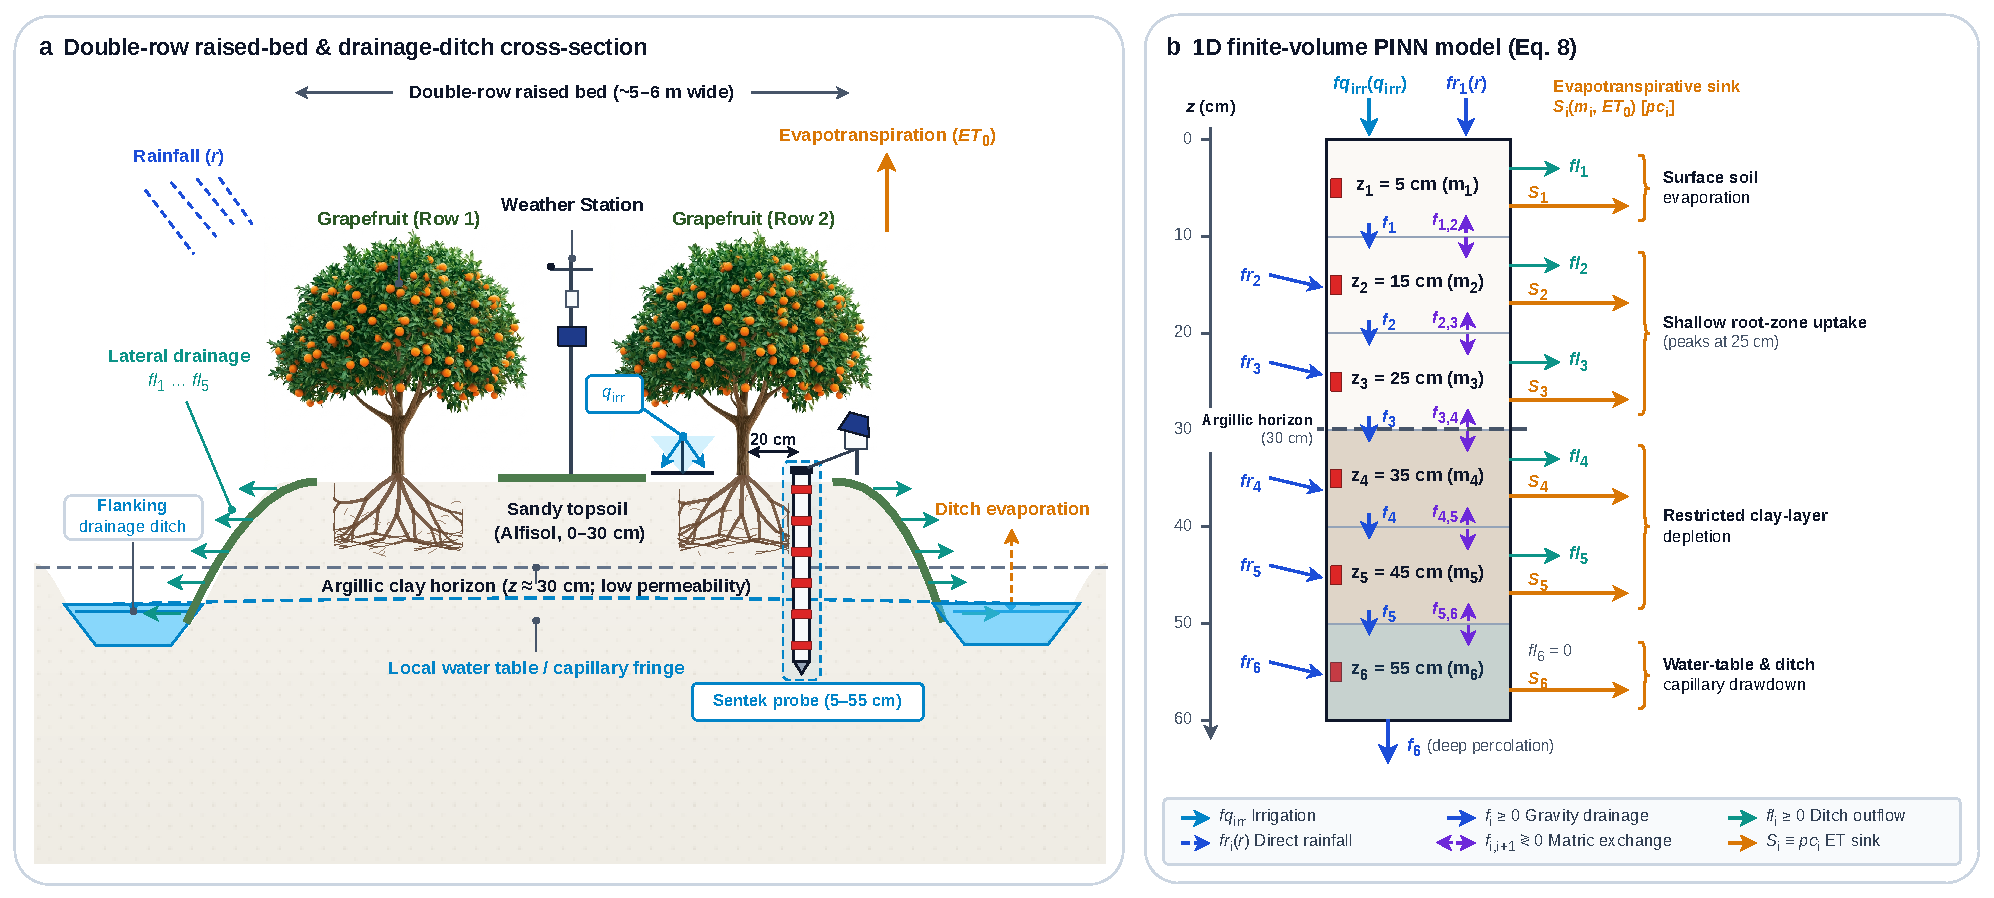
\includegraphics[width=0.92\linewidth]{bed_ditch_schematic.pdf}
\caption{Cross-sectional geometry (not to scale) of the IRREC Millennium Block experimental site (35-acre block; 20-acre active 5,500-tree citrus trial), showing a citrus tree planted on a raised sandy Alfisol bed flanked by drainage ditches above an argillic horizon at $\approx\SI{30}{cm}$ depth. A 6-depth Sentek Drill \& Drop capacitive probe (\SI{20}{cm} from the trunk) monitors 10-\si{cm} vertical compartments centered at 5, 15, 25, 35, 45, and 55~\si{cm}, alongside micro-sprinkler irrigation ($q_{\mathrm{irr}}$), rainfall ($r$), evapotranspiration ($ET_0$), vertical percolation ($f_i$), inter-layer exchange ($f_{i,i+1}$), and lateral ditch drainage ($fl_1\dots fl_5$).}
\label{fig:bed_ditch}
\end{figure}

\begin{figure}[!htbp]
\centering
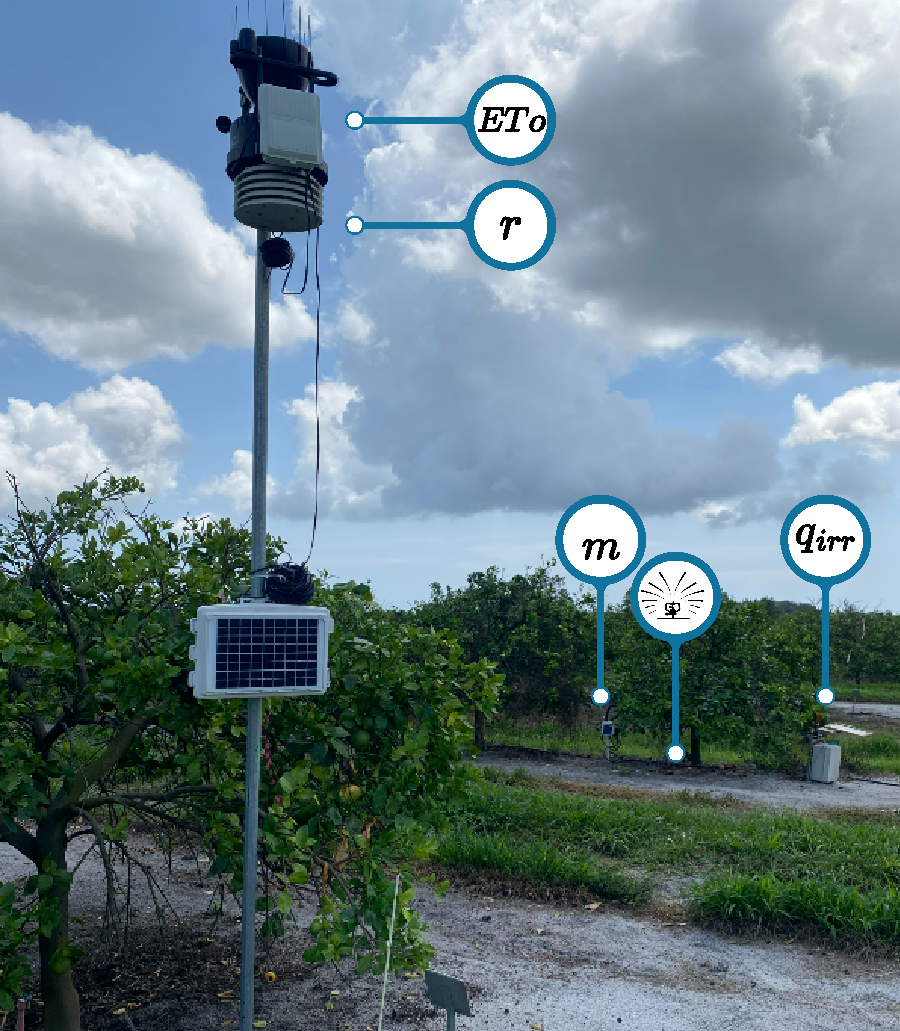
\includegraphics[width=0.5\linewidth]{sensorsmillenniumb.pdf}
\caption{Description of experimental setup, where a weather station, soil moisture probe, and irrigation sensor were deployed to collect soil moisture ($m$), rain ($r$), potential evapotranspiration ($ET_0$), and irrigation ($q_{\mathrm{irr}}$) data.}
\label{sensorsmillennium}
\end{figure}

In a designated section of the Millennium Block, multiple sensors were installed (Fig. \ref{sensorsmillennium}), with data collected, processed, and stored using Irrigmonitor, a custom cloud-based application that facilitates real-time data integration for agricultural water management. The following instrumentation was deployed:
\begin{description}
\item[Weather Station:] A Davis Vantage Pro2 weather station\footnote{See \url{https://www.davisinstruments.com/pages/vantage-pro2} for more information on Davis weather stations.} providing rainfall (\si{mm/h}) and meteorological variables (temperature, humidity, wind speed, solar radiation, and barometric pressure). These data were employed to calculate $ET_0$ (\si{mm/h}) using the FAO-56 Penman--Monteith method \cite{allen1998crop}.
\item[Soil Moisture Probe:] SM measurements ($m_1\dots m_6$ in \si{\%VWC}) were taken at 5\si{cm}, 15\si{cm}, 25\si{cm}, 35\si{cm}, 45\si{cm}, 55\si{cm} using a Sentek Drill \& Drop probe\footnote{Series II Sentek Drill \& Drop probe, capable of measuring SM, temperature, and salinity at 10\si{cm} intervals. See \url{https://sentektechnologies.com/download/sentek-drill-drop-probe-manual/} for details.}, located 20\si{cm} from the base of the tree.
\item[Irrigation Sensor:] Irrigation events were detected by installing two electrodes at the supply irrigation point, connected to a Campbell Scientific CR1000X datalogger, where changes in electrical conduction were used to identify irrigation events and their hourly duration fraction ($q_{\mathrm{irr}} \in [0, 1]\,\si{h/h}$).
\end{description}

The training dataset comprises 840 hourly timestamps spanning 839 elapsed hours ($\approx 35$~days, producing 839 one-hour finite-difference transitions) from March 28, 2025, 21:00:00 to May 2, 2025, 20:00:00, encompassing roughly seven distinct rainfall events and multiple scheduled irrigation cycles (Fig. \ref{Mainfig}). The duration of the training window was selected to ensure a sufficient number of rain events, which are scarce compared to other variables, such as reference evapotranspiration, which changes continuously, or irrigation events, which can be controlled to generate data. Further research on optimizing the estimation window duration and addressing scenarios with limited rainfall is planned, but is beyond the scope of this study.
Raw validation sensor logs span 1,008 hourly records from April 24 to June 5, 2025. To ensure strict temporal separation after training, we extract the held-out 3-day validation benchmark via \(t_{\mathrm{val}} \in [216, 288]\,\si{h}\) (73 hourly records spanning 72 elapsed hours, from May 3, 2025, 21:00:00 to May 6, 2025, 21:00:00), leaving a 25-hour separation buffer before the initial validation state $m(0)$ on May 3 at 21:00:00; the full 792 unseen hours through June 5, 2025, 20:00:00 are evaluated in Section~\ref{sec:benchmarks} across 30 rolling 3-day windows and a 7-day rollout. During all held-out forecasting evaluations, observed station rainfall ($r$), $ET_0$, and irrigation ($q_{\mathrm{irr}}$) series are supplied as known external inputs to isolate intrinsic model dynamics free of numerical weather prediction uncertainty; in live scheduling deployment, operational National Weather Service forecast feeds \cite{NWS2024} replace historical weather inputs. This 3-day validation window aligns with the typical 3-day prediction horizon of weather forecast data from sources such as the National Weather Service \cite{NWS2024}, which can be integrated into the algorithm for predictive irrigation management. This duration assesses the approach's effectiveness in leveraging short-term weather forecasts for irrigation scheduling.
All data were processed and standardized to a one-hour sampling interval to match the temporal resolution of weather forecast data \cite{NWS2024}. This sampling interval was chosen as a constraint because although sensors can collect data at smaller temporal scales, irrigation management strategies that integrate weather forecasts must rely on the temporal resolution of available forecast data.

\subsection{Computational Tools and Algorithm Setup}
The PINN was implemented using TensorFlow 2.10, with 64-bit floating-point precision (\texttt{float64}) to promote numerical stability and accuracy. TensorFlow’s automatic differentiation (synthetic differentiation) was employed to compute gradients and embed physical constraints directly into the training process.
The numerical integration of the PINN’s differential equations was performed using a custom RK4 solver (\(\Delta t = \SI{1}{h}\)) fully integrated into TensorFlow’s computational graph. Randomness across initialization and uniform collocation sampling (\(M = 1{,}000\) points per step) was controlled using fixed seed \texttt{42} across Python, NumPy, and TensorFlow. Both stages used AMSGrad-Adam optimization with gradient norm/value clipping at 0.5 and staircase exponential decay (factor 0.9 every 1,000 steps): Stage~1 ran for 3,000 epochs starting from \(\eta_1 = \num{7.97e-5}\), and Stage~2 refined parameters via RK4 trajectory tracking for 1,000 epochs starting from \(\eta_2 = \num{5.0e-6}\).

% Source code: FINAL_SUBMISSION/code/pinn_training.py (derived from Pinparameb.py)
% Figures: FINAL_SUBMISSION/code/paper_figures.ipynb
% Optuna: optuna_stage1b.py (Stage 1, 200 trials), PINN_optuna_stage2.py (Stage 2, 30 trials)
Hyperparameter optimization was performed using Optuna 3.5, a Bayesian optimization framework, across 200 trials for Stage 1, each evaluated for 150 epochs using the derivative loss ($j_1$), followed by 30 trials for Stage 2. Key hyperparameters obtained included:
\begin{itemize}
\item Initial learning rate for Stage 1 ($\eta_1$): \num{7.97e-5} (and Stage 2 $\eta_2 = \num{5.0e-6}$).
\item Number of neurons per layer ($H$): 56 (with $2H = 112$ on two-input sink branches $S_i$).
\item Loss weight multipliers: $\lambda_{c_1} = \num{113982766}$, $\lambda_{c_2} = \num{1773295}$, and $\lambda_{c_3} = \num{126704656}$.
\end{itemize}

\FloatBarrier

\section*{Funding}
This research was supported by the United States - Israel Binational Agricultural Research and Development Fund (Grant ID IS-5774-25) and the Florida Department of Agriculture and Consumer Services (Grant ID 33200).

\section*{Code availability}
All custom Python/TensorFlow code developed for this study—including the two-stage PINN training pipeline, branched flux-network definitions, custom \texttt{float64} RK4 solver, inference scripts, trained model weights, statistical verification utilities, and the complete benchmark, ablation, and physical admissibility evaluation scripts—is openly deposited in Zenodo at \url{https://doi.org/10.5281/zenodo.19446129}.

\section*{Data availability}
The complete raw and hourly processed field sensor datasets (weather station, multi-depth soil moisture probe, and irrigation conductance telemetry) supporting all training, 3-day benchmark, and rolling unseen-window analyses are publicly deposited in Zenodo at \url{https://doi.org/10.5281/zenodo.19446129}.

\section*{Author contributions}
G.C. conceived the methodology, developed the PINN software and numerical verification experiments, analyzed the field data, and drafted the manuscript. S.M.G. supervised the research, acquired funding, designed the irrigation monitoring infrastructure, and contributed to manuscript revision. J.I.P. contributed to the control-theoretic, system-identification, and optimization formulation and manuscript review. F.T.Z. managed the Millennium Block citrus experimental site, provided agronomic interpretation, and reviewed the manuscript. All authors read and approved the final manuscript.

\section*{Competing interests}
The authors declare no competing interests.

\bibliography{PINN}% common bib file


\end{document}